%=========================================================================
% (c) Michal Bidlo, Bohuslav Křena, 2008


\chapter{Úvod}
Během začátku 21. století došlo k~ohromnému růstu v~oblastech internetu, sociálních sítí, multimédií, chytrých telefonů a~dalších zařízení, či mobilních plateb a~on-line transakcí. V podstatě ve všech oblastech jako je například věda, politika, strojírenství, medicína, doprava, energetika, se nevyhneme použití digitálních zařízení. S~tím velmi úzce souvisí nárůst objemu digitálních dat, která je potřeba ukládat, analyzovat, zpracovávat, a také vyšetřovat.

Digitální zařízení se mohou stát terčem útoků, může se jednat o krádež citlivých dat, podvržení dat, sledování a další. Digitální zařízení mohou být také nástrojem zločinu.

Rozdílnost mezi formáty digitálních dat, jejich strukturované a~nestrukturované vlastnosti, a~také prudký nárůst vyžadují mnoho rozličných přístupů a~technologií pro jejich zpracování.

Cílem této práce je navrhnout a~vytvořit distribuované úložiště pro digitální forenzní data. V~rámci teoretické části práce, se kapitola \ref{chapter1} zaměřuje na forenzní analýzu digitálních dat, vysvětluje, jak probíhá a~co je jejím cílem. Zabývá se také formáty digitálních forenzních dat a~existujícími systémy, které slouží k~uchování těchto dat a~důkazního materiálu. Následně je představen systém AFF4.

Kapitola \ref{chapter2} pojednává o~úložištích pro rozsáhlá strukturovaná i~nestrukturovaná data. V~jejich kontextu vysvětluje také termín Big data. Následují odstavce zaměřeny na distribuované databáze včetně jejich výhod a~nevýhod. Kapitola je završena uvedením principů NoSQL databází, rozdělení podle typů, a srovnání s relačními databázemi. Na NoSQL databázích bude založeno úložiště distribuovaného repositáře.

Cílem praktické části práce je navrhnout a~implementovat distribuovaný repositář. V~kapitole návrhu \ref{distrRepDesignChapter} je vysvětlena architektura systému, aplikační rozhraní, vlastnosti úložišť, princip ovládání repositáře a~také rozšiřitelnost pro nové druhy digitálních forenzních dat. Systém využívá Big data technologie. Pro komunikaci s klientem jsou zprávy přenášeny tzv. \texttt{Message brokerem} Kafka. Jako úložiště slouží, v závislosti na tom, o jaký typ forenzních digitálních dat se jedná, NoSQL databáze a distribuovaný souborový systém HDFS.

Kapitola \ref{chapter_impl} se zabývá implementací distribuovaného úložiště,  technickými detaily, způsobem asynchronní komunikace s databázemi, ukládáním a dotazováním nad daty (sekvenčním i náhodným). Systém pracuje nad frameworkem Spring, který usnadňuje konfiguraci a použití Big data komponent. Jako běhové prostředí byl zvolen projekt \texttt{Docker}, který poskytuje jednotné rozhraní pro izolaci aplikací do kontejnerů.

Poslední kapitola \ref{chapter_performance} se věnuje výkonnosti systému, hardwarovým požadavkům a konfiguraci, a použití systému pro vybrané druhy digitálních forenzních dat.

%Pro ověření základních aspektů návrhu byl také implementován prototyp distribuovaného repositáře, který řeší převážně rozhraní komunikace s~klientem, způsob ovládání repositáře, a~rovněž zpracování požadavků od klienta. Prototypem se zabývá kapitola \ref{chapterPrototype}.

\chapter{Forenzní analýza digitálních dat} \label{chapter1}
Forenzní analýza digitálních dat je věda identifikující, zachovávající, obnovující, analyzující a~předávající fakta ohledně digitálních důkazů nalezených v~počítačích nebo digitálních úložištích mediálních zařízení.
Nezabývá se tedy pouze počítači, ale také ostatními digitálními technologiemi včetně mobilních telefonů a~tabletů, mobilních sítí, internetového bankovnictví, datových médií apod.

Forenzní analýza digitálních dat slouží k získání digitálního důkazního materiálu, který může být použit v soudní síni proti obviněnému. Nalezené výstupy nejsou omezeny k použití pouze u soudu. Častokrát může nějaká firma řešit interní záležitosti jako například porušení firemní politiky, kdy se zase musí najít (digitální) důkaz, který potvrzuje nebo vyvrací obvinění.

Pod výše uvedenými aktivitami se skrývá \cite{whatIsDigFor}:

\begin{itemize}
\item Identifikace - Jedná se o~první část celého procesu. Předtím, než je cokoliv zkoumáno a~analyzováno, je důležité identifikovat, kde jsou data uložena. Typicky jsou uložena na diskových jednotkách, serverech, flash klíčenkách, síťových zařízeních.

\item Zachování - Důležitá je ochrana důkazů, tzn. pro sběr a~analýzu informací je potřeba zachovat původní data, musí se zabránit jejich změně a~ztrátě. Bez integrity je důkazní materiál nepoužitelný. Identifikovaná původní data mohou být zajištěna chronologickým řetězcem dokumentů (anglicky \texttt{chain of custody}), který zaznamenává veškeré aktivity s digitálním důkazem jako je přenos, úschova, kontrola a stav.

\item Obnovení - Součástí procesu je i~obnova dat, která může zahrnovat obnovu smazaných dat procesy operačního systému, úmyslně smazané soubory, soubory chráněné heslem a~také poškozené soubory. I po obnovení smazaného souboru musí být stále zachována integrita.

\item Analýza - Jedná se o~hlavní část vyšetřování. Cílem je shromáždit co nejvíce relevantních artefaktů. Prohledávána je paměť, registry, výpisy z logů aplikací, historie internetového prohlížeče apod. Podstatná je i dokumentace všech kroků, které byly provedeny.

\item Předání - Po analýze jsou artefakty důkladně zdokumentovány a~odevzdány například ve formě protokolu. Po shromáždění všech nalezených informací může ale nemusí dojít k definitivnímu rozhodnutí. Co se s informacemi stane už není v rukou vyšetřovatele. Tady proces forenzní analýzy končí.
\end{itemize}

\noindent Vyšetřování digitálních forenzních dat obvykle zahrnuje vytvoření forenzní duplikace zkoumaného média. Provádí se proto, aby se neznehodnotil původní zdroj. Například dojde k vytvoření obrazu disku, který je kopie celého disku nebo jeho části bit po bitu. Neduplikuje se celý systém, pokud je prostor příliš velký. Obraz je statický snímek, který může být analyzován za účelem odhalení nebo stanovení událostí ohledně incidentů, a~může tak být použitý jako důkaz v~soudní síni. Analýza je prováděna na kopii pro zachování integrity originálu.

Vyšetřovatel zanalyzuje obraz pomocí snímacích technik, aby získal relevantní data z~disku. Forenzní obraz obsahuje soubory z~disku, ale také nealokovaný prostor a~tzv. \texttt{slack space}. Slack space je pozůstatek diskového prostoru, který byl alokován pro nějaký počítačový soubor a~ten všechen prostor nepotřebuje. Právě v~těchto prostorech mohou být nalezeny relevantní artefakty a informace jako například smazané soubory, či jejich fragmenty \cite{forensicImages}.

\begin{figure}[!h]
  \centering
  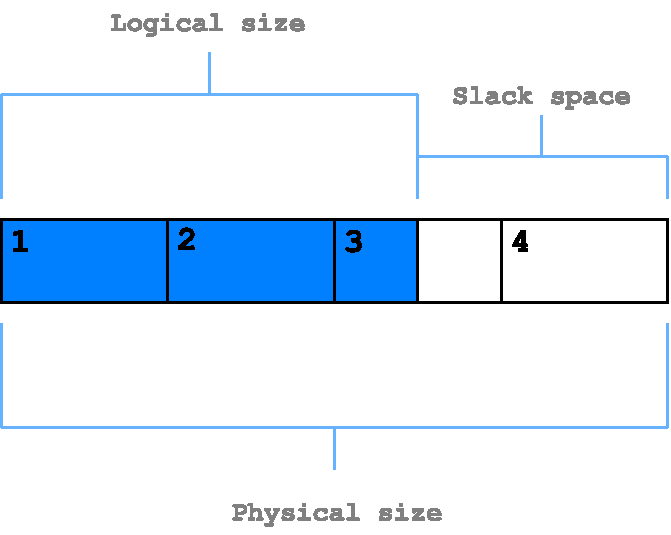
\includegraphics[width=10.5cm]{template-fig/SlackSpace.pdf}
  \caption{Příklad znázorňuje slack space pro parametry: sektory velikosti 512 bajtů v operačním systému jsou shluknuty do skupin po čtyřech, tzn. velikost svazku je 2048 bajtů; velikost souboru je 1280 bajtů (modrá barva). Pro tento soubor byl alokován celý svazek 2048 bajtů, nevyužité místo je slack space, v tomto případě se jedná o 768 bajtů \cite{slacSpace}.}
  \label{FIG_SlackSpace}
\end{figure}

\section{Formáty digitálních forenzních dat}
Typů digitálních forenzních dat existuje spousta. Každý typ takových dat může být reprezentován jiným formátem. Tato sekce čerpá informace převážně z~\cite{forensicswikiForensicFF}.

Mnoho forenzních počítačových programů používají své vlastní formáty pro uložení informace. Můžeme je rozdělit na nezávislé (anglicky \texttt{Independent File Formats}) a~programově specifické formáty (anglicky \texttt{Program-Specific File Formats}):

\begin{itemize}
\item Nezávislé - Tyto formáty byly vyvinuty nezávisle na konkrétním forenzním programu. Patří mezi ně \texttt{AFF}, \texttt{AFF4}, \texttt{gfzip}, \texttt{Raw Image Format}.

\item Programově specifické - Byly vyvinuty pro použití specifickými forenzními programy. Většinou každý takový formát je unikátní, a~proto je pro přečtení potřeba unikátního nástroje.
Zástupci jsou například \texttt{Encase image file format}, \texttt{ProDiscover image file format}, \texttt{IXimager file formats}.
\end{itemize}

\subsubsection{Identifikace formátu}
%File Format Identification
Identifikace formátu souboru je proces určení formátu nějaké sekvence bajtů. Operační systém toto typicky dělá rozpoznáním přípony souboru nebo podle zabudované \texttt{MIME} informace. Forenzní aplikace musí identifikovat typy souborů podle obsahu. Mezi existující systémy patří například tyto projekty \--\ \texttt{libmagic}, \texttt{PRONOM}, \texttt{Apache Tika} \footnote{http://tika.apache.org/} \cite{forensicswikiFFIdentification}.

\section{Existující systémy}
Vyznamným zástupcem pro uložení digitálních forenzních dat je systém AFF4, který bude popsán detailněji.

\subsection{AFF4}
Jedná se o~open source formát pro ukládání digitálních důkazů a~dat. Jeho výhodami jsou správa metadat a~možnost komprese. Tato sekce čerpá převážně z~\cite{aff4}. Je založen na objektově orientované architektuře. Veškerá množina známých objektů je označována jako \texttt{AFF4 universe}. Takový prostor je definovaný jako nekonečný, protože AFF4 je navržen pro škálování obrovského množství důkazního materiálu. Všechny objekty jsou adresovatelné jejich jménem, které je v~rámci AFF4 universe unikátní.

\vspace{0.5cm}

\noindent Příkladem jména nějakého AFF4 objektu může být:

\texttt{urn:aff4:f3eba626-505a-4730-8216-1987853bc4d2}

\noindent Jedná se o~standardní URN notaci, URN je unikátní.

\vspace{0.5cm}

\noindent AFF4 universe používá RDF notaci pro specifikaci atributů objektů. V~nejjednodušší podobě je RDF množina tvrzení o~objektu ve formátu:

\texttt{Subject   Attribute   Value}

\vspace{0.5cm}

\noindent Příklad:

\noindent \texttt{******** Object urn:aff4:f3eba626-505a-4730-8216-1987853bc4d2 ***********}\\
\texttt{aff4:stored = urn:aff4:4bdbf8bc-d8a5-40cb-9af0-fd7e4d0e2c9e}\\
\texttt{aff4:type = image}\\
\texttt{aff4:interface = stream}\\
\texttt{aff4:timestamp = 0x49E9DEC3}\\
\texttt{aff4:chunk\_size = 32k}\\
\texttt{aff4:compression = 8}\\
\texttt{aff4:chunks\_in\_segment = 2048}\\
\texttt{aff4:size = 10485760}\\

\noindent Příklad ukazuje, že objekt má tyto atributy a~hodnoty. Nazýváme je relace nebo fakta. Celý AFF4 universe je sestavený z~takových faktů.

\noindent AFF4 objekty existují, protože dělají něco užitečného, což závisí na rozhraní, které představují. Aktuálně existuje několik rozhraní, nejvýznamnější jsou \texttt{Volume} a~\texttt{Stream}. Rozhraní objektu je fakt o~objektu, který nalezneme v~atributu \texttt{aff4:interface}.

\subsubsection{Rozhraní Volume}
Rozhraní Volume definujeme jako mechanismus ukládání, který dokáže uložit segment (bit binárních dat) pod nějaké jméno, a~získat jej podle tohoto jména. Aktuálně existují dvě implementace: \texttt{Directory} a~\texttt{ZipFile}.

\begin{itemize}
\item \texttt{Directory Volume} - Tato implementace ukládá segmenty jako soubory uvnitř běžného adresáře v~souborovém systému. Hodí se zejména, pokud potřebujeme uložit obraz na souborový systém FAT, přičemž velikost segmentu je malá a~nenarazíme tak na omezení velikosti souboru. Je také možné založit adresář na nějaké http adrese, což nám umožní používat obraz přímo z~webu.

\item \texttt{ZipFile Volume} - Jak napovídá název, tato implementace ukládá segmenty uvnitř zip archivu. Malé soubory lze bez problémů otevřít obyčejným průzkumníkem (windows explorer) a~data extrahovat. Zase je možné zapsat zip archiv přímo na HTTP server a~používat obraz přímo ze serveru.
\end{itemize}

\noindent Je možné převádět mezi oběma formáty z~jednoho na druhý, extrahovat zip archiv do adresáře a~vytvoření Directory volume.

\subsubsection{Rozhraní Stream}
Streamy jsou základním rozhraním pro ukládání dat obrazu. Stream obsahuje metody typu \texttt{read}, \texttt{seek}, \texttt{tell} a~\texttt{close}. Podporuje ještě \texttt{write}, ale ne k~modifikaci obrazu, nýbrž k~jeho vytvoření (kvůli výše uvedené integritě zdroje). Pokud nějaký AFF4 objekt podporuje rozhraní stream, lze provést náhodné čtení jeho dat. Existuje několik specifických implementací rozhraní stream, některými z~nich jsou:

\begin{itemize}
\item \texttt{FileBackedObjects} - Stream, který ukládá data v~souboru v~souborovém systému, jehož pozice je určena URN souboru.

\item \texttt{HTTPObject} - Pozice souboru je udána pomocí URL. Objekt lze ukládat a~číst z~HTTP serveru. Implementace umožňuje přečíst určité rozmezí bajtů. Režie síťového provozu mezi klientem a~serverem je minimální. Je možné vyšetřit vzdálený obraz přes HTTP bez potřeby celé kopie obrazu. Z důvodu bezpečnosti by měl být server pro zápis nějak omezen, například hesly, SSL certifikáty apod. Podpora čtení může být poskytnuta bez omezení, pokud je zdroj dat zašifrován. Zabezpečení serveru je ale mimo rozsah AFF4.

\item \texttt{Segments} - Segmenty jsou komponenty uloženy přímo ve \texttt{Volume}. Volume je zjednodušeně řečeno objekt uchovávající segmenty. Segmenty by měly být použity pro malé streamy, protože prohledávat v~komprimovaných segmentech může být drahá operace. Segmenty jsou užitečné, pokud potřebujeme vytvořit logický obraz nějaké podmnožiny souborového systému (pouze některé soubory) a~ne forenzní obraz celkového systému.
% Hodí se v situacích kdy je souborový systém příliš velký, a víme, že většina obsahu není relevantní. 

\item \texttt{Image streams} - Tyto streamy jsou opakem segmentů. Pro velké obrazy nemůžeme použít segmenty, protože by nebyly zkomprimovány efektivně. Image stream ukládá obraz v~tzv. \texttt{chunks}.
\end{itemize}

\chapter{Úložiště pro rozsáhlá strukturovaná i~nestrukturovaná data} \label{chapter2}
V~této kapitole bude představen a~vysvětlen termín Big data, následován systémy a~mechanismy pro uložení, jako například distribuované databáze a~NoSQL databáze, včetně jejich vlastností, výhod a~nevýhod.

\section{Big data} \label{bigDataSection}
Definicí pro frázi Big data existuje několik. Jedná se o~termín použitý na soubory dat, které jsou příliš komplexní z~hlediska velikosti a~různorodosti, a~které je nemožné zpracovávat běžně používanými přístupy a~softwarovými nástroji v~rozumném čase.

Objem takových dat rychle roste. Vyskytují se v~mnoha odvětvích, například sběr informací o~počasí, sociální sítě, energetické a~telekomunikační společnosti, ekonomie a~finančnictví, či data z~kamer, měření z~různých senzorů apod. Z~toho plyne, že se jedná o~data různorodých typů, mohou být strukturovaná i~nestrukturovaná. Proto je potřeba existence různých technologií pro jejich uložení, zpracování, analýzu i~zobrazení.

%\begin{figure}[!h]
%  \centering
%  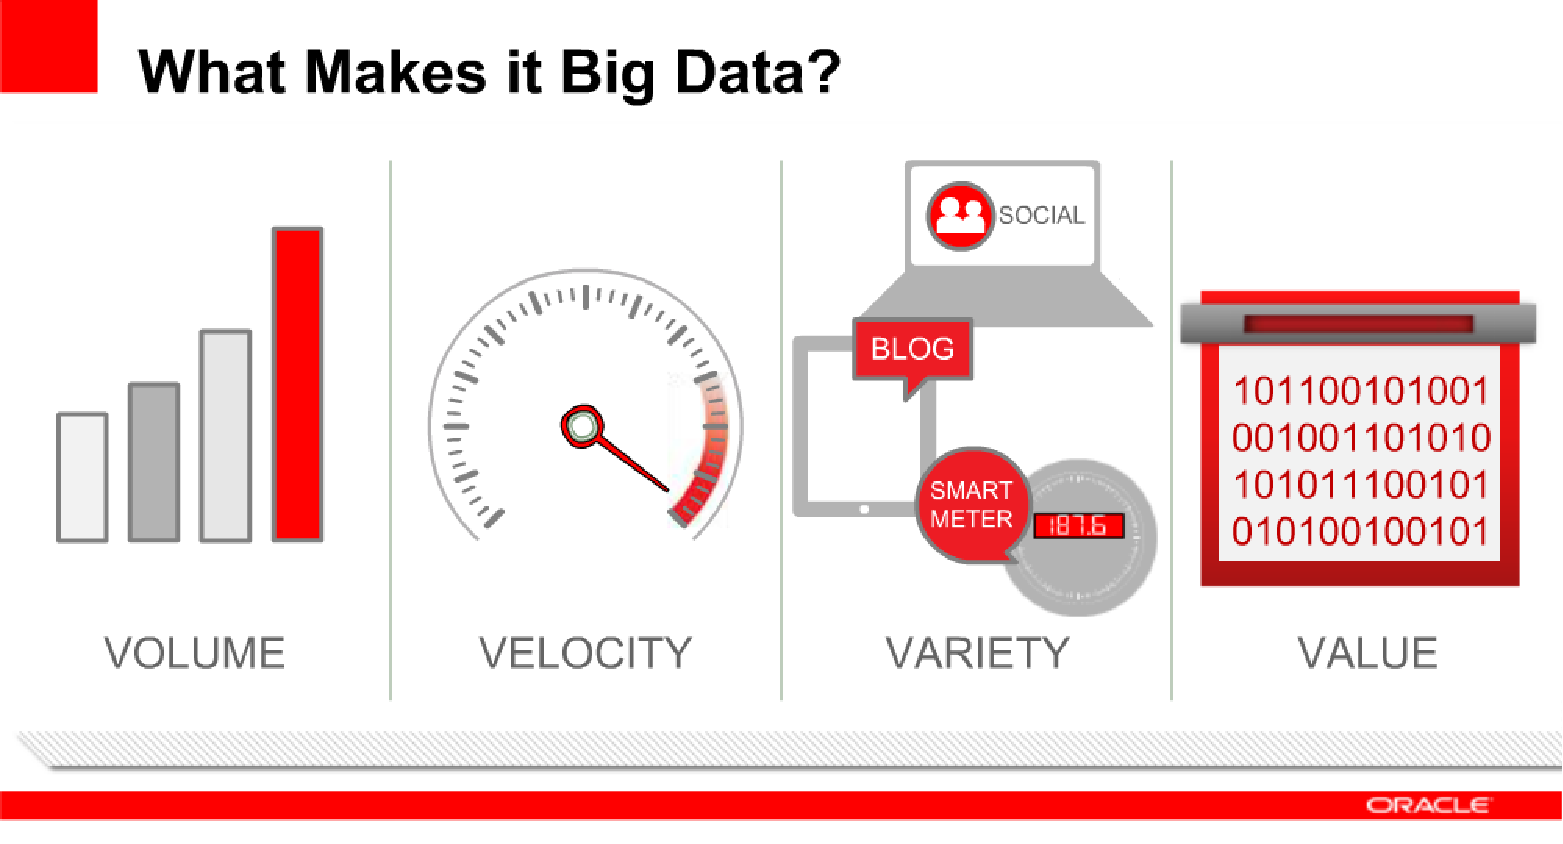
\includegraphics[width=12.5cm]{template-fig/what_makes_data_big_data.pdf}
%  \caption{Definice Big data podle Oracle. \cite{johanBigData}}
%  \label{FIG_BigData}
%\end{figure}

\vspace{0.5cm}

\noindent Pojem Big data je často definován jako 4V z~anglických slov Volume, Velocity, Variety a~Value \cite{oracleBigData}:

\begin{itemize}
\item Volume – Značí množství nebo velikost dat. Je vyžadováno zpracování vysokých objemů dat neznámých hodnot, například síťový provoz, data sesbírána ze senzorů apod.

\item Velocity – Vyjadřuje rychlost z~hlediska vzniku dat a~potřeby jejich analýzy, některá vyžadují zpracování v~reálném čase. Nejdůležitější data se zapisují přímo do paměti, a~ne na disk, z~důvodu co nejrychlejšího zpracování.

\item Variety – Znamená různorodost typů. Jedná se především o~nestrukturovaná data, například text, audio, video, data o~geografické poloze a~další. Jsou na ně kladeny velmi podobné požadavky jako na data strukturovaná – sumarizace, monitorování, důvěrnost \cite{oracleBigData}.

\item Value – Data mají vlastní hodnotu, která musí být analyzována a~zjištěna. Nejedná se o~jednoduchý proces, je stále potřeba nových metod a~technik zpracování.
\end{itemize}

\begin{figure}[!h]
  \centering
  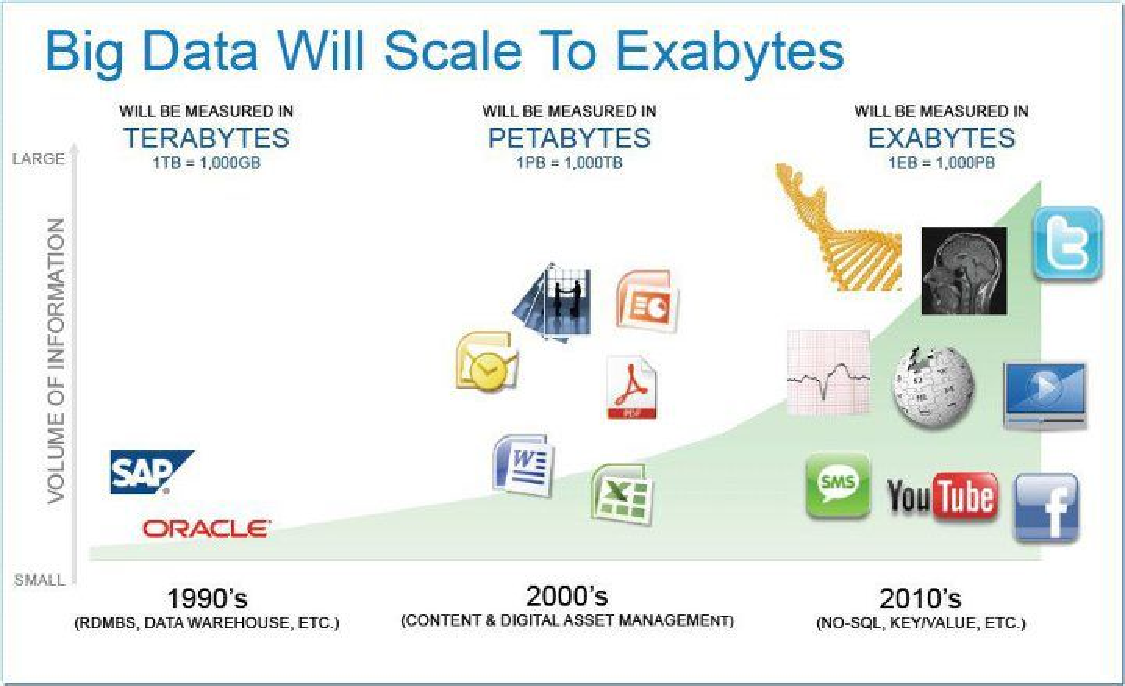
\includegraphics[width=15cm]{template-fig/big_data_exabytes.pdf}
  \caption{S~přibývajícími novými technologiemi se masivně zvyšuje růst dat a~přibývají nové typy \cite{rajeshBigData}.}
  \label{FIG_BigDataExabytes}
\end{figure}

%\noindent Tato práce se zabývá Big daty hlavně typu – PCAP soubory, logy ze síťových zařízení a komunikací. Možnosti uložení Big data budou popsány v následujících podkapitolách.

\section{Distribuované databáze}
Distribuovaná databáze se skládá z~většího počtu samostatných databází, které mohou být geograficky rozmístěny na jiných pozicích. Jednotlivé uzly spolu komunikují přes počítačovou síť. Každý uzel je sám o~sobě databázový systém. DSŘBD neboli systém řízení distribuované báze dat (anglicky Distributed Database Database Management System) zajišťuje, že se distribuovaná databáze uživatelům jeví jako jedna jediná databáze. Data jsou fyzicky uložena na různých pozicích. Mohou být spravována rozdílnými SŘBD nezávisle na ostatních pozicích.

\vspace{0.5cm}

\noindent Systém řízení distribuované báze dat je centralizovaný systém s~těmito vlastnostmi 
\cite{distributedDBMS}:

\begin{itemize}
\item Umí vytvářet, získávat, upravovat a~mazat distribuované databáze.

\item Zajišťuje důvěrnost a~integritu databází.

\item Periodicky synchronizuje databázi a~poskytuje mechanismy přístupu tak, aby se databáze uživatelům jevila transparentní.

\item Zajišťuje, že změna dat v~kterémkoliv uzlu se promítne i~v~ostatních uzlech.

\item Je využíván v~aplikacích, kde se předpokládá zpracování velkých objemů dat, ke kterým přistupuje současně mnoho uživatelů.

\item Je navržen pro heterogenní databázové platformy.
\end{itemize}

\begin{figure}[!h]
  \centering
  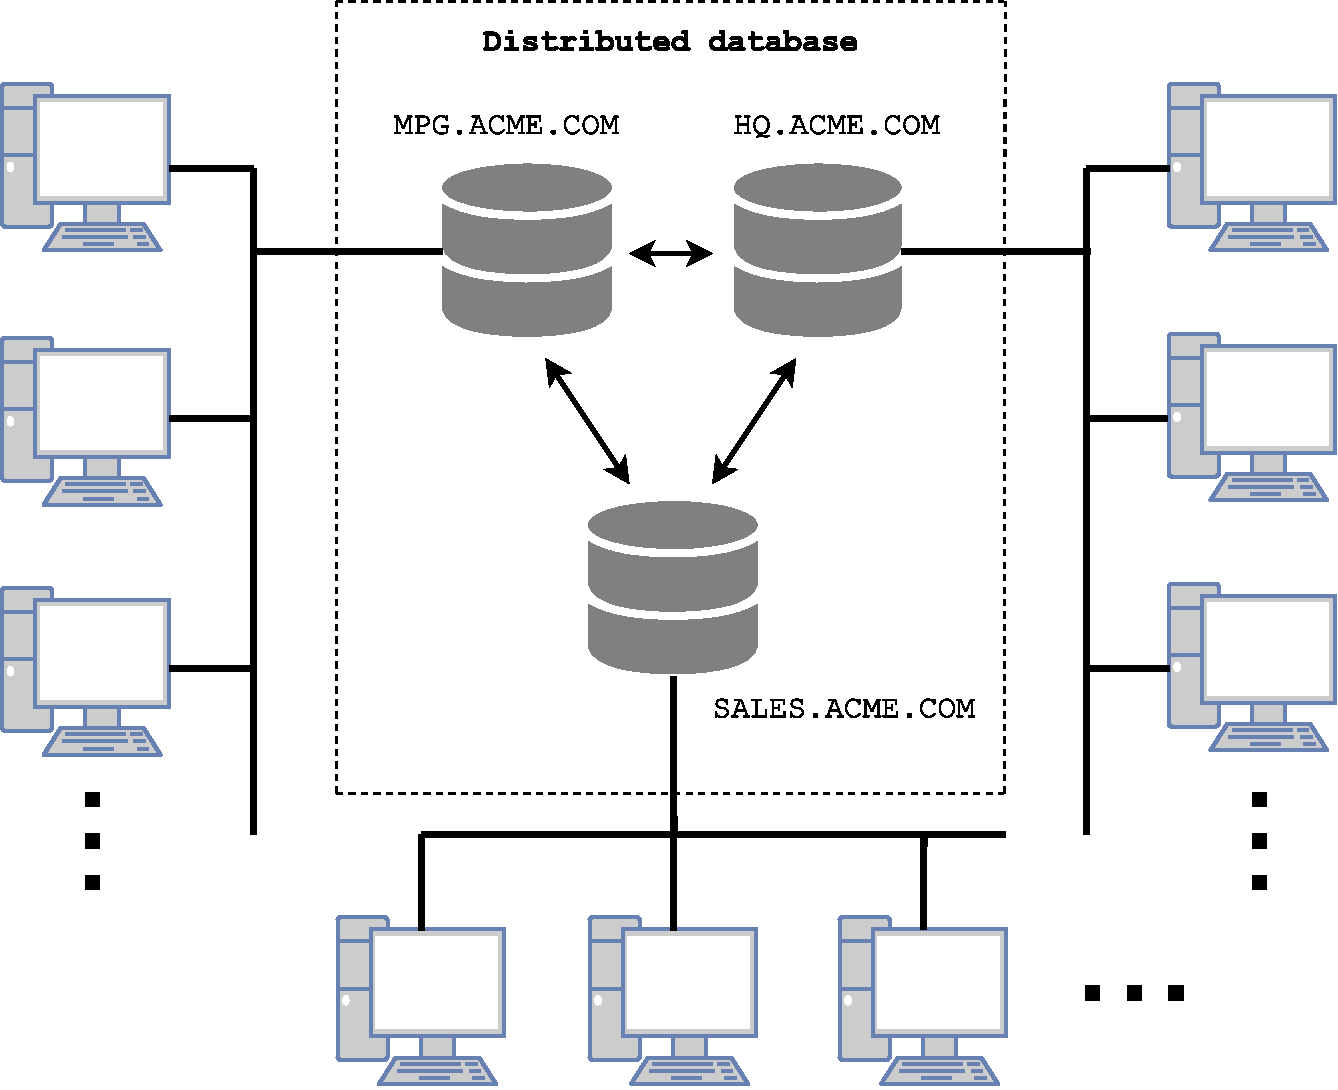
\includegraphics[width=13cm]{template-fig/DistributedDatabase.pdf}
  \caption{Schéma distribuované databáze a~současný přístup více zařízení k~ní \cite{distributedDBMSPic}.}
  \label{FIG_DistrDB}
\end{figure}

\noindent Výhody
\begin{itemize}
\item Rozšiřitelnost – Pokud je potřeba databázový systém rozšířit do nových míst nebo přidat další uzly, stačí přidat nový(é) počítač(e) a~lokální data v~nové pozici, a~nakonec je připojit k~distribuovanému systému, bez jakéhokoliv přerušení funkcionality. Analogický postup je při odebrání uzlu.

\item Spolehlivost – Když nějaký z~připojených uzlů selže, nepřestane distribuovaná databáze fungovat, sníží se maximálně výkon.

\item Ochrana (záloha) dat – Při zničení jednoho uzlu a~smazání dat z~něj, mohou být stejná data zálohována i~na jiných uzlech.

\item Výkonnost – Pokud jsou data efektivně distribuována, může být uživatelův požadavek uspokojen rychleji. Transakce mohou být také distribuované a~provedeny rychleji. 
\end{itemize}

\noindent Nevýhody
\begin{itemize}
\item CAP teorém - Pojednává o tzv. eventuální konzistenci (na rozdíl od absolutní konzistence u ACID). Definuje, že distribuovaný systém může zajistit maximálně 2 z těchto 3 vlastností: konzistence (angl. Consistency), dostupnost (angl. Availability) a odolnost k přerušení (angl. Partition tolerance). Je nutné si zvolit mezi konzistencí a dostupností v případě výpadku části sítě.

\item Integrita dat – Data musí být průběžně synchronizována na více uzlech, aby na stejné dotazy nebyly z~různých uzlů vraceny rozdílné odpovědi.

\item Komunikační režie – I~zdánlivě jednoduchá operace může vyžadovat spoustu zbytečné komunikace.

\item Cena – DSŘDB vyžaduje drahý a~složitý software ke koordinaci uzlů a~zajištění transparentnosti \cite{distributedDBMS}.

\item Mezi další patří – složitost, zabezpečení, řízení souběžného přístupu k~datům.
\end{itemize}

\begin{figure}[!h]
  \centering
  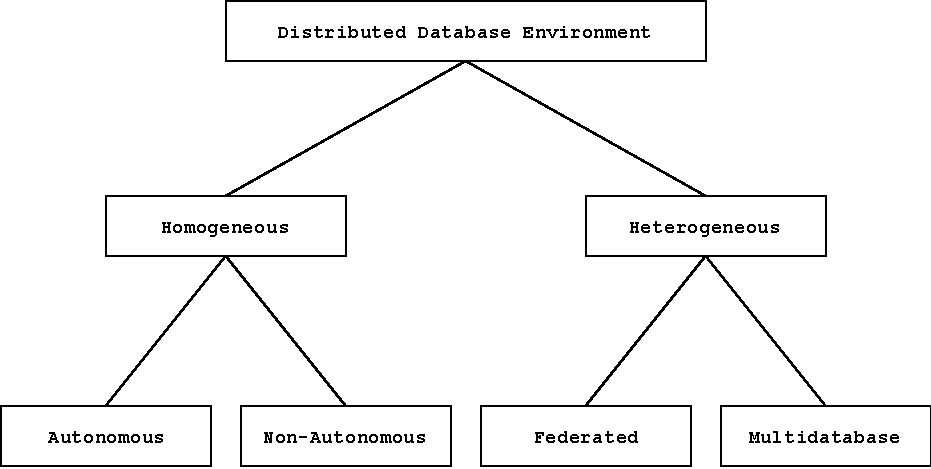
\includegraphics[width=14.2cm]{template-fig/DistributedDatabasesClassification.pdf}
  \caption{Distribuované databáze můžeme podle jejich vlastností dělit \cite{distributedDBMS}.}
  \label{FIG_DivDistrDB}
\end{figure}

\subsection{Rozdělení}
\subsubsection{Homogenní}
Všechny uzly používají identické SŘBD a~operační systémy. Uzly mají informace o~ostatních uzlech a~spolupracují při zpracování uživatelských požadavků. Homogenní distribuovaná databáze se navenek jeví uživateli jako jeden systém. Je jednodušší jej navrhnout a~spravovat.

\vspace{0.5cm}
\noindent Autonomní - Každá databáze je nezávislá, neexistuje žádný centrální uzel. Databáze jsou spravovány aplikací, a~pro předávání dat používají zasílání zpráv.

\vspace{0.5cm}
\noindent Neautonomní - Data jsou distribuována napříč homogenními uzly. O~aktualizaci a~správu dat se stará systém řízení distribuované báze dat, který běží na centrálním nebo také master uzlu.

\subsubsection{Heterogenní}
Uzly mohou mít rozdílné operační systémy a~SŘBD, které nejsou kompatibilní. Mohou také využívat rozdílná schémata (relační, objektově orientované, hierarchické, \ldots). Rozdílnost schématu je hlavním problémem při zpracování dotazu a~transakcí. Kvůli tomu je také složité dotazování \cite{wikiDBMS}. Heterogenní distribuované databáze můžeme rozdělit na federované (angl. federated) nebo multidatabázové.

\vspace{0.5cm}
\noindent Architekturami distribuovaných databází jsou centrální architektura, klient-server, peer-to-peer, a multi-databázová architektura.

\section{Úložiště}
V~této sekci budou popsána strukturovaná a~nestrukturovaná data, jaký je mezi nimi rozdíl a~jaká jsou jejich úložiště.

\subsection{Strukturovaná data}
Strukturovanými daty jsou libovolná data, pro která lze sestavit datový model. Datový model přesně organizuje jednotlivé elementy dat a~specifikuje, jak spolu elementy souvisí, jaké mají vazby, jak budou uloženy, přístup k~nim, a~jak souvisí s~jednotlivými elementy reálného světa \cite{structData}. Typickým úložištěm strukturovaných dat je relační databáze. Pro čtení a~dotazování byl vytvořen dotazovací jazyk SQL.

\subsection{Nestrukturovaná data}
Jak už bylo zmíněno v~sekci \ref{bigDataSection}, Big data patří převážně mezi nestrukturovaná data. Data nemají přesně definovanou strukturu, neexistuje datový model, který by definoval jednotlivé dílčí elementy a~jejich vztahy. Mezi typické zástupce patří: videa, obrázky, audio, webové stránky, text, obsah e-mailové komunikace apod. Mezi vhodná úložiště mohou patřit disková úložiště, NAS (celým názvem \texttt{Network Attached Storage}), HDFS (\texttt{Hadoop Distributed File System}) a~NoSQL databáze.

\subsubsection{NoSQL databáze}
Pod zkratkou se nachází \texttt{non SQL} nebo také \texttt{Not only SQL}. Jedná se o~databázový koncept, ve kterém datové úložiště i~zpracování dat používají jiné prostředky než tabulková schémata tradiční relační databáze \cite{noSqlWiki}. NoSQL databáze jsou navrženy pro distribuovaná ukládání a~dotazování dat, souběžný přístup, a~manipulaci s~obrovským objemem dat. Mezi výhody patří: horizontální i~vertikální škálovatelnost, distribuovaný přístup, flexibilita schématu, dynamičnost. Nevýhodami však mohou být: absence standardizace, omezené schopnosti dotazování, konzistence \cite{noSqlIntro}.

\vspace{0.5cm}
\noindent NoSQL databáze mohou být rozděleny do čtyř kategorií \cite{noSqlOverview}:
\begin{itemize}
    \item Klíč-hodnota (angl. Key-Value databases) - Jsou nejjednoduššími NoSQL úložišti. Každá položka v~databázi je uložena jako atribut (klíč) společně se svou hodnotou. Hodnota je typu \texttt{blob}, takže pouze aplikace dokáže hodnotu správně interpretovat. Databáze pouze ukládá binární data, kterým nerozumí. Klíč může být složený, např. z několika částí, které lze použít jako ID do struktury a ID jejich položek. Klíče mohou být seřazené, což umožňuje efektivní procházení, nebo také organizovány do hierarchií. Zástupci jsou databáze \texttt{Riak} a~\texttt{Redis}.
    
    \item Dokumentové (angl. Document databases) - Párují každý klíč se složitou datovou strukturou, nazývanou dokument. Představuje v podstatě princip klíč-hodnota, ale hodnota je strukturovaná. Dokument může obsahovat mnoho rozdílných párů klíč-hodnota, párů klíč-pole, nebo dokonce vnořené dokumenty. Jsou vhodné pro dokumenty formátu XML a~JSON (BSON).
    Databáze dokáže interpretovat strukturovanou hodnotu (dokument), toho lze efektivně využít hlavně při dotazování. Dotazy mohou být i složitější než přes klíče, např. pomocí XPath. Mezi zástupce patří \texttt{MongoDB} a~\texttt{CouchDB}.
    
    \item Grafové (angl. Graph databases) - Jsou navrženy pro ukládání entit (uzly) a~jejich vztahů (hrany). Uzly i~hrany mohou mít svoje atributy. Jsou vhodné pro reprezentaci sítí a jejich topologií, např. sociální či dopravní sítě, topologie počítačových sítí a~další \cite{noSqlPdb}.
    Zástupcem je \texttt{Neo4J}.
    
    \item Sloupcové (angl. Column-oriented databases / Column family stores) - Organizace dat v tabulkách. Tabulka má řádky jako v relační databázi, ale u řádku pak lze definovat sloupce s hodnotami. Sloupce mohou být pro každý řádek různé (flexibilní schéma), i různý počet (řídké pole). Sloupcové databáze jsou optimalizovány pro dotazování nad velkými objemy dat. Sloupce mohou být zobecněny na adresáře (anglicky \texttt{supercolumn}), kde potom řádek obsahuje kolekci supersloupců, a z nich každý obsahuje kolekci sloupců \cite{noSqlPdb}. Zástupci sloupcových databází jsou například \texttt{Cassandra} a~\texttt{HBase}.
\end{itemize}

\subsection{Srovnání relačních a NoSQL databází}
Podle výše uvedených vlastností úložišť pro strukturovaná a nestrukturovaná data můžeme vidět tyto rozdíly:

\begin{multicols}{2}

Relační databáze

\begin{itemize}
    \item Datový model je formalizovaný, databáze umožňuje definovat integritní omezení, kontroly, model reflektuje elementy reálného světa.
    
    \item S daty lze provádět transformace v podobě spojení, agregací, řazení apod.
    
    \item Kvůli podpoře transakcí a ACID vlastností není úplně snadná škálovatelnost.
    
    \item Mají pevné schéma databáze. Vzniklé problémy po úpravách se musí řešit např. migračními skripty.
\end{itemize}

\columnbreak

NoSQL databáze

\begin{itemize}
    \item Jedná se o nízkoúrovňové úložiště, kde ve většině případů databáze není schopna data interpretovat. Zajištění konzistence je ponecháno aplikaci. 
    
    \item Data lze dostat pouze v podobě, v jaké byla uložena.
    
    \item Jsou navrženy pro jednoduchou škálovatelnost.
    
    \item Mají dynamické schéma, které neomezuje definovat libovolnou strukturu a provádět flexibilní úpravy.
\end{itemize}

\end{multicols}

\chapter{Návrh distribuovaného úložiště} \label{distrRepDesignChapter}
Tato kapitola se zabývá návrhem distribuovaného úložiště rozsáhlých digitálních forenzních dat. Bude popsána architektura systému včetně aplikačního rozhraní a~použité technologie pro vytvoření distribuovaného repositáře.
Systém bude založen na Big data technologiích - Kafka (společně se ZooKeeper), NoSQL databáze a HDFS ze systému Hadoop. Jak jednotlivé technologie fungují bude vysvětleno v~této kapitole.

\section{Aplikační rozhraní}
Aplikační rozhraní umožňuje klientovi komunikovat s~distribuovaným repositářem. Komunikace je založena na asynchronním zasílání zpráv. Systém repositáře nenabízí klientovi přímo žádné metody či funkce, které by klient mohl volat. Ovládání repositáře probíhá pomocí zaslání zprávy obsahující tzv. příkaz. Příkaz specifikuje typ operace a typ dat. Podle typu příkazu je určeno, jak se daný příkaz zpracuje. V~následující sekci bude vysvětleno, jak ovládání repositáře probíhá, jak vypadá zpráva, a~bude také uvedeno schéma celé komunikace jako příklad.

\subsection{Komunikace} \label{designCommunication}
Komunikace s~klientem, který chce do distribuovaného repositáře data uložit, nebo naopak z~něj nějaká data získat, probíhá pomocí zaslání zprávy tzv. \texttt{MQ broker}u Kafka. Zpráva obsahuje parametry - atributy příkazu a~případně řetězec dat. Atributy příkazu udávají následující informace:

\begin{itemize}
    %\item \texttt{operation} - o~jakou operaci se jedná, výchozí operace jsou \texttt{SAVE}, \texttt{LOAD},
    
    %\item \texttt{dataType} - typ dat,  výchozími typy jsou \texttt{Text}, \texttt{PCAP}, \texttt{Packet},
    
    \item \texttt{command} - určuje typ příkazu, příklady příkazů mohou být \texttt{STORE\_PCAP} a \texttt{LOAD\_PCAP}. Příkaz v sobě ještě zapouzdřuje typ operace, které mohou být \texttt{SAVE} a \texttt{LOAD}, a také typ dat jako například \texttt{PCAP}, \texttt{Packet}, \texttt{BINARY}, \texttt{LOG} apod.
    
    \item \texttt{id} - unikátní ID zprávy, aby klient potom dokázal identifikovat už zpracované příkazy.
    
    \item \texttt{awaitsResponse} - jestli klient/odesilatel zprávy očekává od repositáře odpověď.
    
    \item \texttt{responseTopic} - ve které frontě (angl. topic) je odpověď na straně klienta očekávána.
    
    \item \texttt{errorTopic} - na straně distribuovaného úložiště se může vyskytnout chyba, například nedostupnost databáze, chyba při zpracování příkazu a další. Tento parametr slouží pro zadání fronty, kam se budou zasílat chybová hlášení.
    
    \item \texttt{dataSource} - zdrojová data k uložení lze zaslat dvojím způsobem. První z nich je poslat data v binární podobě přímo přes systém Kafka společně s příkazem. Tento způsob lze využít pro data, jejichž velikost není příliš velká, protože se data načítají do paměti RAM. Pro velké objemy dat takový přístup není vhodný. Proto existuje ještě druhý způsob, a to předat data přes distribuovaný souborový systém HDFS. Parametr dataSource obsahuje název úložiště v podobě výčtové konstanty \texttt{Kafka} nebo \texttt{HDFS}, cestu k souboru, pokud se jedná o HDFS, a také atribut \texttt{removeAfterUse} pro odstranění souboru po použití.
    
    \item \texttt{criterias} - seznam kritérií pro dotazování. Tento parametr je vhodné vyplnit pouze pro operace čtení.
\end{itemize}

\noindent Řetězec dat obsahuje vlastní data, která mají být na straně repositáře zpracována. Typy příkazů, a v podstatě typy operací s typy dat lze libovolně přidávat.

\begin{figure}[!h]
  \centering
  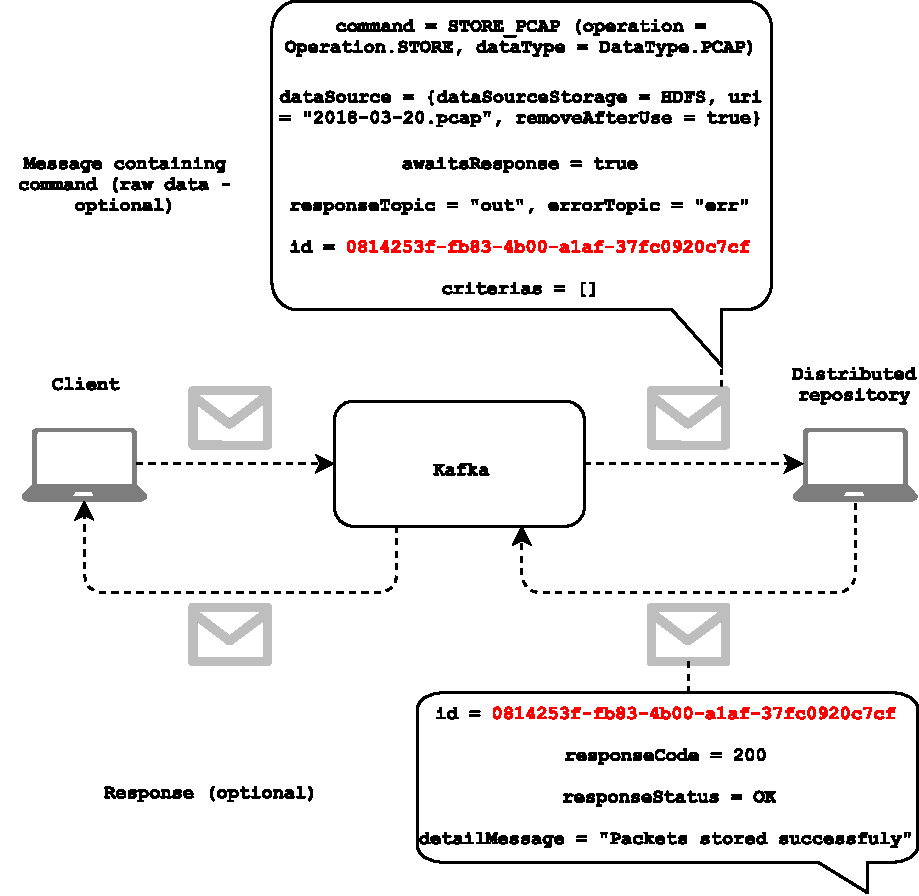
\includegraphics[width=14.1cm]{template-fig/Kafka_communication.pdf}
  \caption{Demonstrace komunikace - zaslání příkazu pro uložení souboru PCAP. Klient zašle příkaz přes Kafku, příkaz je zpracován na straně distr. repositáře, a~případně je odeslána odpověď klientovi. Můžeme si všimnout uvedených ID, jsou stejné - klient zjistí, ke kterému příkazu odpověď patří.}
  \label{FIG_KafkaCommunication}
\end{figure}

\subsection{Kafka}
Apache Kafka je distribuovaný systém zpráv s~robustními frontami založený na mechanismu \texttt{publish-subscribe} umožňující přenášet vysoké objemy dat. Kafka zprávy jsou perzistentně uloženy na disku a~replikovány v~rámci clusteru kvůli prevenci ztráty dat. Framework Kafka je postaven na synchronizační službě ZooKeeper \cite{kafkaTutorialsPoint}.

\vspace{0.5cm}
\noindent Výhody jsou:
\begin{itemize}
    \item Spolehlivost - Kafka je distribuovaný systém, segmentovaný, replikovaný a~odolný proti chybám.
    \item Rozšiřitelnost - Možnost připojení nových uzlů do clusteru.
    \item Odolnost - Zprávy jsou uloženy na disku.
    \item Výkon - Vysoká propustnost pro obě akce \texttt{publish} a~\texttt{subscribe}. Je zachován stabilní výkon i~při objemu zpráv v~terabytech.
\end{itemize}

\begin{figure}[!h]
  \centering
  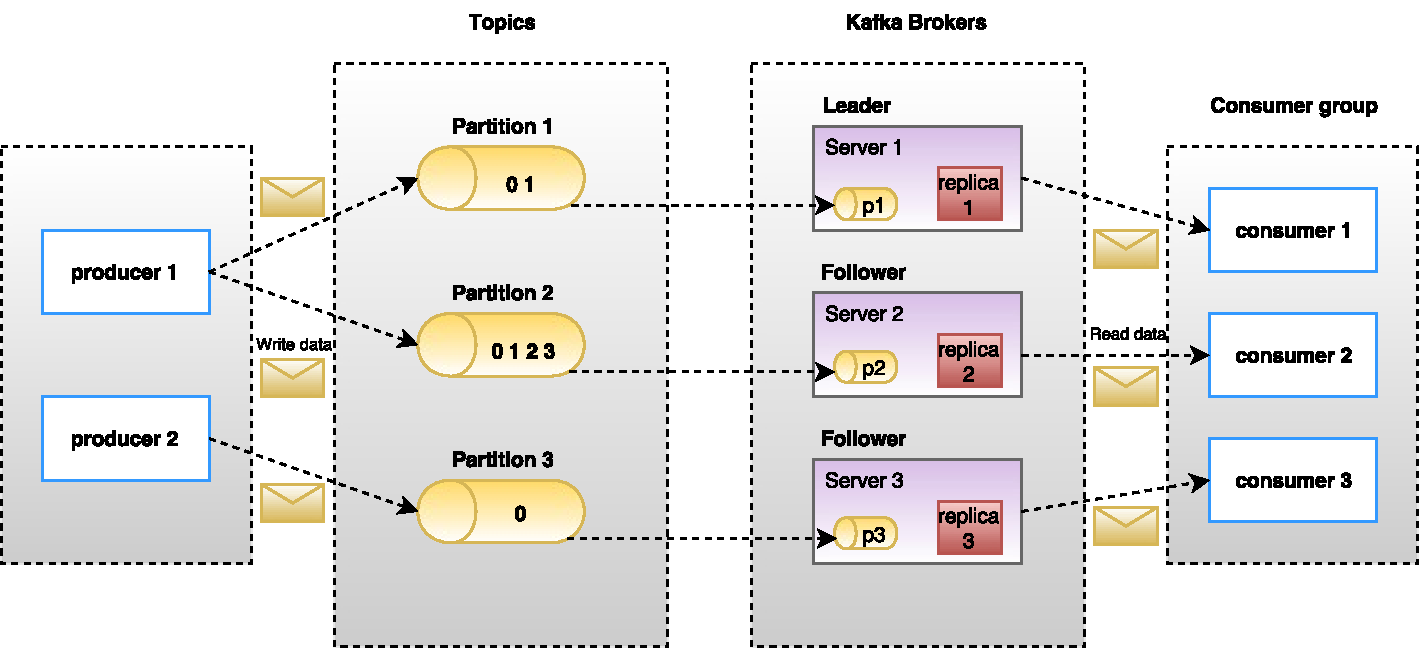
\includegraphics[width=15cm]{template-fig/Kafka_architecture.pdf}
  \caption{Diagram zobrazující klíčové komponenty systému Kafka \cite{kafkaTutorialsPoint}.}
  \label{FIG_KafkaArchitecture}
\end{figure}

\noindent V~diagramu \ref{FIG_KafkaArchitecture} je fronta (angl. topic) konfigurována do tří oddílů (angl. partition). Pokud je faktor replikace fronty nastaven na hodnotu 3, Kafka vytvoří tři identické repliky každého oddílu a~umístí je do clusteru. Každý prostředník (angl. broker) ukládá jeden nebo více těchto oddílů za účelem vyvažování zátěže. Více producentů, respektive konzumentů, může zároveň vydávat (angl. publish), resp. odebírat, (angl. subscribe) zprávy \cite{kafkaTutorialsPoint}.

\vspace{0.5cm}
\noindent Hlavní komponenty systému Kafka z~diagramu \ref{FIG_KafkaArchitecture}:
\begin{itemize}
    \item Fronta - Jedná se o~proud zpráv patřící k~příslušné kategorii. Data jsou uložena ve frontách. Fronty jsou rozděleny do oddílů.
    
    \item Oddíl - Fronty mohou mít mnoho oddílů, tak aby zvládaly zpracování libovolného množství dat.

    \item Offset oddílu (angl. Partition offset) - Každá zpráva v~oddílu má unikátní sekvenci ID nazývanou offset.

    \item Replika oddílu - Je pouhou zálohou oddílu. Repliky nejsou využívány ke čtení nebo zápisu dat, slouží pouze jako prevence před ztrátou dat.
    
    \item Prostředník - Jednoduchý systém zodpovědný za správu dat v~oddílech, resp. frontách. Prostředníci slouží k~balancování zátěže.
    
    \item Kafka Cluster - Pokud existuje víc než jeden prostředník, pak se systém nazývá cluster. Cluster může být rozšířen bez prodlev o~další prostředníky.
    
    \item Producent - Je odesilatel zprávy do jedné nebo více Kafka front. Producenti posílají data prostředníkům. Pokaždé když producent pošle zprávu prostředníkovi, prostředník přidá zprávu na konec oddílu. Producent nečeká na žádná potvrzení, posílá zprávy tak rychle, jak jen prostředník dokáže přijímat.
    
    \item Konzument - Čte data od prostředníka(ů). Odebírá z~jedné nebo více front a~konzumuje zprávy vytažením dat od prostředníků.
\end{itemize}

\section{Úložiště}
Tato sekce se zaměřuje na úložiště, kde budou digitální forenzní data uchována. Můžeme je rozdělit na strukturovaná a~nestrukturovaná.

\subsection{Strukturovaná data}
V~souvislosti se systémem repositáře se obecně jedná o~data, která mohou být rozdělena na menší části při zachování možnosti interpretace, a~mohou být efektivně serializována pro uložení. Mezi strukturovaná data můžeme zařadit například soubory formátu \texttt{PCAP} obsahující síťovou komunikaci. Tyto soubory lze rozparsovat na jednotlivé segmenty pakety. Pakety lze potom serializovat na pole bajtů a~uložit do NoSQL databáze. Pro strukturovaná data byla vybrána databáze Cassandra.

\subsubsection{Cassandra}
Jedná se o~zástupce sloupcových NoSQL databází. Výhodami jsou předně: škálovatelnost, odolnost proti chybám, rychlost, distribuovanost, konzistence a~podpora transakcí. Cassandru využívají i~světoznámé společnosti Facebook, Twitter, Cisco, ebay, Twitter, Netflix a~další. Cílem Cassandry je zvládat vysoké objemy dat napříč mnoha uzly. Data jsou pak distribuována na všech uzlech clusteru. Uzly lze libovolně přidávat. Každý uzel je nezávislý a~zároveň propojený s~ostatními. Každý uzel v~clusteru se může podílet na požadavcích čtení a~zápisu nezávisle na tom, kde jsou data skutečně uložena. Když uzel selže, požadavky čtení a~zápisu mohou být obslouženy jinými uzly sítě \cite{cassandraTutorialsPoint}.

\subsection{Nestrukturovaná data}
Pro uchování nestrukturovaných dat typu například audio, video, logů, a obecně binárních dat bude sloužit distribuovaný souborový systém HDFS. Taková data mohou mít velký objem, a~bylo by plýtvání výkonem provádět jejich serializaci nebo rozdělování na části při ukládání do NoSQL databází.

\subsubsection{Hadoop a HDFS}
Distribuovaný souborový systém HDFS patří pod projekt \texttt{Apache Hadoop}, který je navržen pro ukládání a zpracování obrovského množství dat v distribuovaném prostřední napříč mnoha počítači. Počítá se škálovatelností od jednoho serveru po tisíce strojů, kde každý z nich nabízí lokální úložiště a výpočetní zdroje \cite{hadoopTutorialsPoint}.

\vspace{0.5cm}
\noindent Platforma Hadoop zahrnuje tyto moduly:

\begin{itemize}
    \item \texttt{Hadoop Common} - Knihovny a pomocné nástroje požadované ostatními Hadoop moduly. Poskytují abstrakce souborového a operačního systému potřebné pro jazyk Java, a skripty nutné pro spuštění Hadoop-u.
    
    \item \texttt{Hadoop YARN} - Jedná se o framework pro plánování distribuovaných úloh a správu zdrojů.
    
    \item \texttt{HDFS} - Distribuovaný souborový systém poskytující vysokou propustnost přístupu k aplikačním datům, škálovatelnost, odolnost proti chybám a efektivní správu zdrojů.
    
    \item \texttt{Hadoop MapReduce} - Systém pro paralelní zpracování obrovského množství vstupních dat. Tento modul je pro systém distribuovaného úložiště zbytečný.
\end{itemize}

\noindent Kromě výše uvedených modulů existují i další pomocné nástroje:  \texttt{Apache Spark}, \texttt{Apache HBase} - distribuovaná databáze, \texttt{Apache Hive} - nástroj pro dolování dat nad platformou Hadoop, \texttt{Apache Pig} atd.

\begin{figure}[!h]
  \centering
  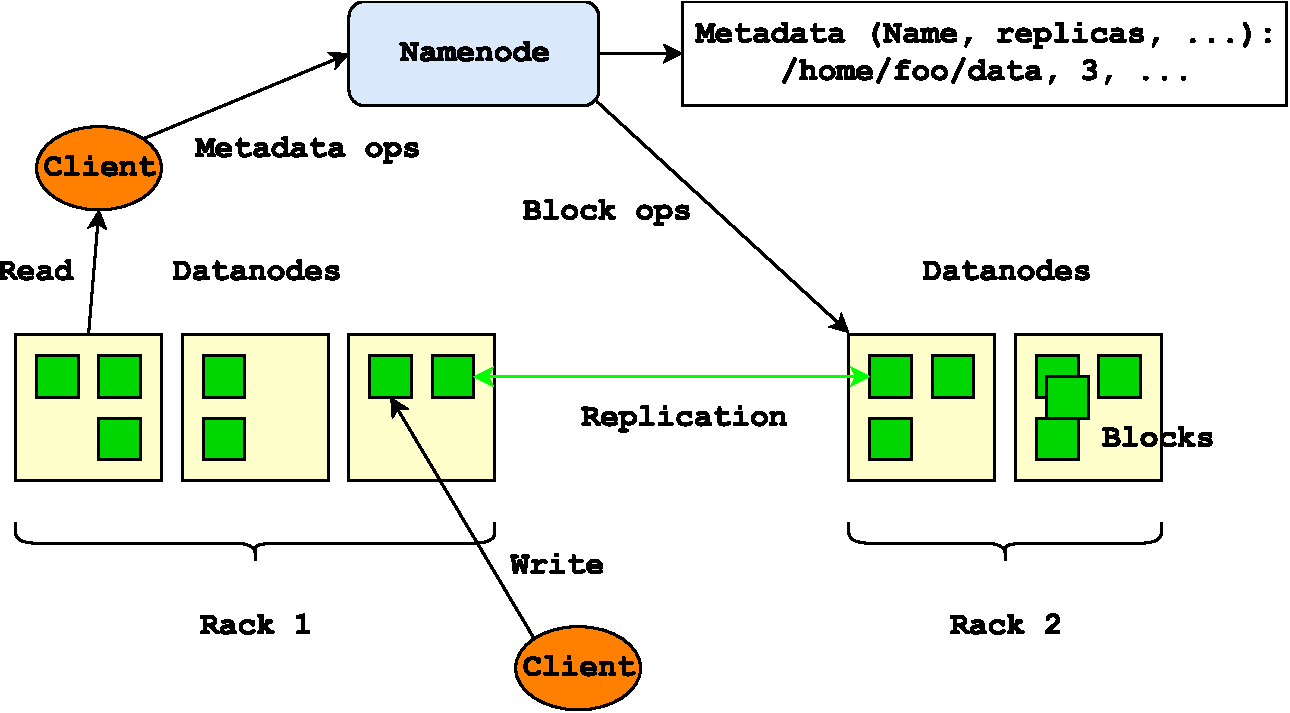
\includegraphics[width=15cm]{template-fig/HDFSArchitecture.pdf}
  \caption{Architektura HDFS \cite{apacheHDFSGuide} - datové uzly jsou uspořádány do \texttt{racků}, které se nachází v jedné lokalitě, což zajišťuje rychlejší propojení uzlů. Bloky jsou replikovány mezi odlišné uzly.}
  \label{FIG_SystemArchitecture}
\end{figure}

\noindent HDFS je virtuální souborový systém vybudovaný nad běžnými souborovými systémy jednotlivých uzlů. Řeší problém nalezení úložiště a přístupu k datům, nikoliv fyzické uložení na uzlu. Byl navržen pro sekvenční přístup k souborům, nikoliv náhodný \cite{hadoopPdi}.

\noindent HDFS používá architekturu typu \texttt{master/slave}. Master se skládá z jednoho uzlu nazývaného \texttt{NameNode}, který se stará o správu metadat a jmenného prostoru souborového systému. Dále reguluje přístup k souborům a provádí operace typu otevření, zavření, přejmenování souborů a adresářů. Protože je NameNode pouze jeden, měl by být spolehlivý a výkonný, při jeho výpadku způsobí poruchu systému (jde o tzv. \texttt{single point of failure}). Uzlů typu slave může být více, jsou nazývány datové uzly (angl. \texttt{DataNodes}), a ukládají data. Soubor je rozdělen do několika bloků (typicky po 64 nebo 128 MB), a každý blok souboru je nezávisle replikován v několika datových uzlech slave. Bloky jsou uloženy v lokálním souborovém systému na datových uzlech. Datové uzly jsou také zodpovědné za zpracování požadavků čtení a zápisu od klientů. NameNode se stará o mapování bloků datovým uzlům, sleduje počet replik jednotlivých bloků. Pokud se nějaká replika ztratí vinou selhání datového uzlu, je vytvořena nová replika bloku \cite{hadoopHortonworks}.

HDFS je implementován v jazyce Java, na každém stroji s nainstalovanou Javou může běžet NameNode nebo DataNode software. Typicky při nasazení existuje jeden stroj s běžícím NameNode, na dalších strojích potom běží datové uzly (lze ovšem najít i scénáře, kde na jednom stroji běží více datových uzlů). Důležité je, že uživatelská data nikdy neprochází přes NameNode \cite{apacheHDFSGuide}.

HDFS poskytuje rozhraní přes příkazovou řádku jako ostatní souborové systémy, které umožňuje interagovat se souborovým systémem.

\subsection{Metadata} \label{metadata}
V~rámci zpracování příchozí zprávy do repositáře informující o~operaci uložení, by bylo vhodné provést předzpracování dat za účelem vhodnější indexace a~rychlejšího nalezení pro budoucí operace čtení. Jednalo by se tak o~mechanismus podobný například pamětem cache. Uvažme následující scénář pro podrobnější vysvětlení.

Do repositáře bylo v~průběhu několika dnů uloženo mnoho milionů paketů, které obsahovaly síťovou komunikaci mezi několika komunikujícími stranami. Data paketů jsou uložena v~serializované podobě v~NoSQL databázi. Na úrovni databáze nedávají taková data žádný význam, pouze aplikace je dokáže správně interpretovat jako pakety. Po několika dnech by uživatel rád zjistil podrobnější informace o~komunikaci mezi uzly A~a~B. Nezbývalo by mu nic jiného, než všechna data z~NoSQL databáze načíst na aplikační úrovni a~analyzovat paket po paketu, aby zjistil minimálně IP adresy zdroje a~cíle. Takový způsob by byl velmi pomalý a~neefektivní.

Následně uvažme, jak by vypadal postup pro zjištění informací o~komunikaci mezi uzly A~a~B, kdyby byla k~dispozici cache, či paměť metadat. Cache by mohla uchovávat základní informace o~dříve uložených paketech v~jednotně definované struktuře. Mezi tyto informace by patřily - zdrojová a~cílová IP adresa, zdrojová a~cílová MAC adresa, typ protokolu, časové razítko a~další. Co je však důležité, u~těchto informací by bylo uvedeno ID záznamu z~NoSQL databáze, kde je uchován celý paket. Pro zjištění podrobnějších informací by uživatel mohl načíst pouze ty pakety, které jsou pro něj relevantní.

Předzpracování dat je výhodné před jejich uložením, protože v~kontextu provádění aplikace jsou data interpretovatelná. Výtah základních informací z~nich nezpůsobí propad výkonu. Naopak se výkon zvýší pro případné operace čtení a~hledání.

Výše uvedený princip by se dal zobecnit pro libovolný typ forenzních digitálních dat. Tak by došlo k~vytvoření tzv. registru, který by i~mimo jiné informoval, co je jak a~kde uloženo. Vhodnou strukturou pro uložení těchto metadat může být například formát XML nebo JSON. Z~toho vyplývá použití dokumentové NoSQL databáze jako například MongoDB.

\subsubsection{MongoDB}
MongoDB je multiplatformní, dokumentově orientovaná databáze poskytující vysoký výkon a~dostupnost a~jednoduchou škálovatelnost. Pracuje na principu kolekcí, které nevyžadují schéma. Kolekce je skupina MongoDB dokumentů, a~je ekvivalentem SŘBD tabulek. Dokumenty v~kolekcích mohou mít dynamická schémata a~rozdílné atributy. Dynamické schéma znamená, že dokumenty ve stejné kolekci nemusí mít stejnou strukturu atributů. Počet atributů, obsah a~velikost dokumentu se může mezi dokumenty lišit. Dokument je množina párů klíč-hodnota \cite{mongoDBTutorialsPoint}.

Relační databáze má určité schéma skládající se z~tabulek a~vztahů mezi nimi. V~MongoDB je koncept vztahu řešen jinak. Existují dva mechanismy umožňující aplikaci reprezentovat vztahy: reference a~vnořené dokumenty. Reference uchovávají vztahy mezi daty vložením odkazů (referencí) z~jednoho dokumentu do druhého. Aplikace může díky odkazu přistoupit k~příslušným datům. Vnořené dokumenty zachycují vztahy mezi daty ukládáním příslušných dat přímo do jednoho dokumentu. Namísto atributu dokumentu může být uložen i~jiný dokument. Výhoda tohoto modelu je, že aplikace získá všechna data v~jedné databázové operaci \cite{mongoDBDataModelingIntro}.

Dynamičnost MongoDB je vhodná pro správu metadat, zvlášť když bude do repositáře potřeba přidávat nové druhy dat.

\section{Jádro distribuovaného úložiště}
V~předchozích sekcích byla představena komunikace s~repositářem, jak vypadají příkazy a~jakým způsobem jsou posílána data. Následně byly popsány možnosti ukládání. Tato sekce se zaměřuje na jádro distribuovaného repositáře, převážně na zpracování příkazů a~manipulaci s~databázemi.

Přijetí příkazu zajišťuje konzument zpráv. Konzument se v~krátkých časových intervalech dotazuje na zprávy z~Kafka fronty. Po přijetí zprávy dojde k~přečtení příkazu určeného typem operace a~typem dat společně s~dodatečnými parametry uvedenými v \ref{designCommunication}. Na základě příkazu dojde k~výběru konkrétní obsluhy (tzv. \texttt{handler}), která má za úkol zpracování příkazu. Může se jednat o~uložení dat, o~načtení dat podle zadaných parametrů, přečtení metadat apod. Handler ukrývá všechny potřebné operace, které mají proběhnout při zpracování příkazu. Mimo jiné se jedná i~o~správu metadat zmíněnou v~sekci \ref{metadata}. Při implementaci budou handleru nastaveny potřebné objekty pro řešení databázových operací pro daný typ dat. Každý typ úložiště (souborový systém nebo NoSQL databáze) může mít jiné rozhraní přístupu.

Důležitým požadavkem je, aby úložiště umožňovalo přidávání podpory pro nové druhy forenzních dat za běhu. Tento požadavek je implicitně zajištěn systémem Kafka, který každou přijatou zprávu zapíše na disk a zpráva tam zůstává, dokud ji konzument úspěšně nezpracuje. V tom případě lze systém repositáře zastavit, ale Kafka zprávy bude pořád přijímat. Mezitím může proběhnout doimplementování nové funkcionality pro jiný druh forenzních dat, provést kompilaci, nasazení a spuštění systému. Po spuštění se konzument začne dotazovat Kafky na nové nepřijaté zprávy.

%TODO: Vice Kafka front? - Vice konzumentu?

\section{Architektura} \label{archSection}
Tato sekce se zabývá architekturou systému, jak bude repositář implementován. Diagram tříd \ref{FIG_SystemArchitecture} zobrazuje z~důvodu přehlednosti pouze klíčová rozhraní a~třídy systému. Nejsou zde vyznačeny všechny implementační třídy a~všechny vazby závislosti.

Tok začíná ve třídě \texttt{DistributedRepository}, která zapouzdřuje konzumenta Kafka front a~správce všech handlerů. Konzument přijme zprávu z~fronty, sestaví objekt příkazu na základě typu operace a~typu dat, a~vybere podle něj korespondující handler ze správce handlerů. Handler potom zpracuje příkaz. V~rámci zpracování může být odeslána asynchronní odpověď klientovi, pokud klient nastavil při odeslání zprávy parametry \texttt{awaitsResponse} a~\texttt{responseTopic}. Odpověď může obsahovat základní informace jako například kód a~status, a~také ID, aby si klient dokázal spárovat zpracované zprávy.

Rozšíření v~podobě podpory nových druhů digitálních forenzních dat je velmi jednoduché. Spočívá v~rozšíření výčtů \texttt{Command}, \texttt{Operation} a~\texttt{DataType}. Dále je potřeba implementovat rozhraní \texttt{IConsumerHandler}, které kompletně řídí zpracování příkazu.
Pro nový druh dat a~potřeby komunikace s~úložištěm nebo databází je nutné přidat implementaci rozhraní \texttt{IStore} a/nebo \texttt{ILoad}.
Nová třída handleru musí být přidána do správce handlerů společně s~typem příkazu.

Díky tomu že jsou typ operace a~typ dat výčty, nemůže klient poslat libovolný dotaz na úplně neznámá data. Příkaz je ale určen kombinací těchto dvou výčtů, a~proto i~tak lze odeslat nepodporovaný příkaz, který může skončit chybou.

Všechny výše zmíněné technologie, tzn. Kafka, Cassandra, MongoDB, i~HDFS, jsou distribuované, je možné přidávat další uzly pro navýšení výkonu, a~všechny tak počítají s~rozšiřitelností do budoucna.

Konfigurace parametrů systému a~jednotlivých technologií bude možná pomocí specifických souborů s~příponou \texttt{.properties} skládajících se z~dvojic klíč-hodnota.

\begin{figure}[!h]
  \centering
  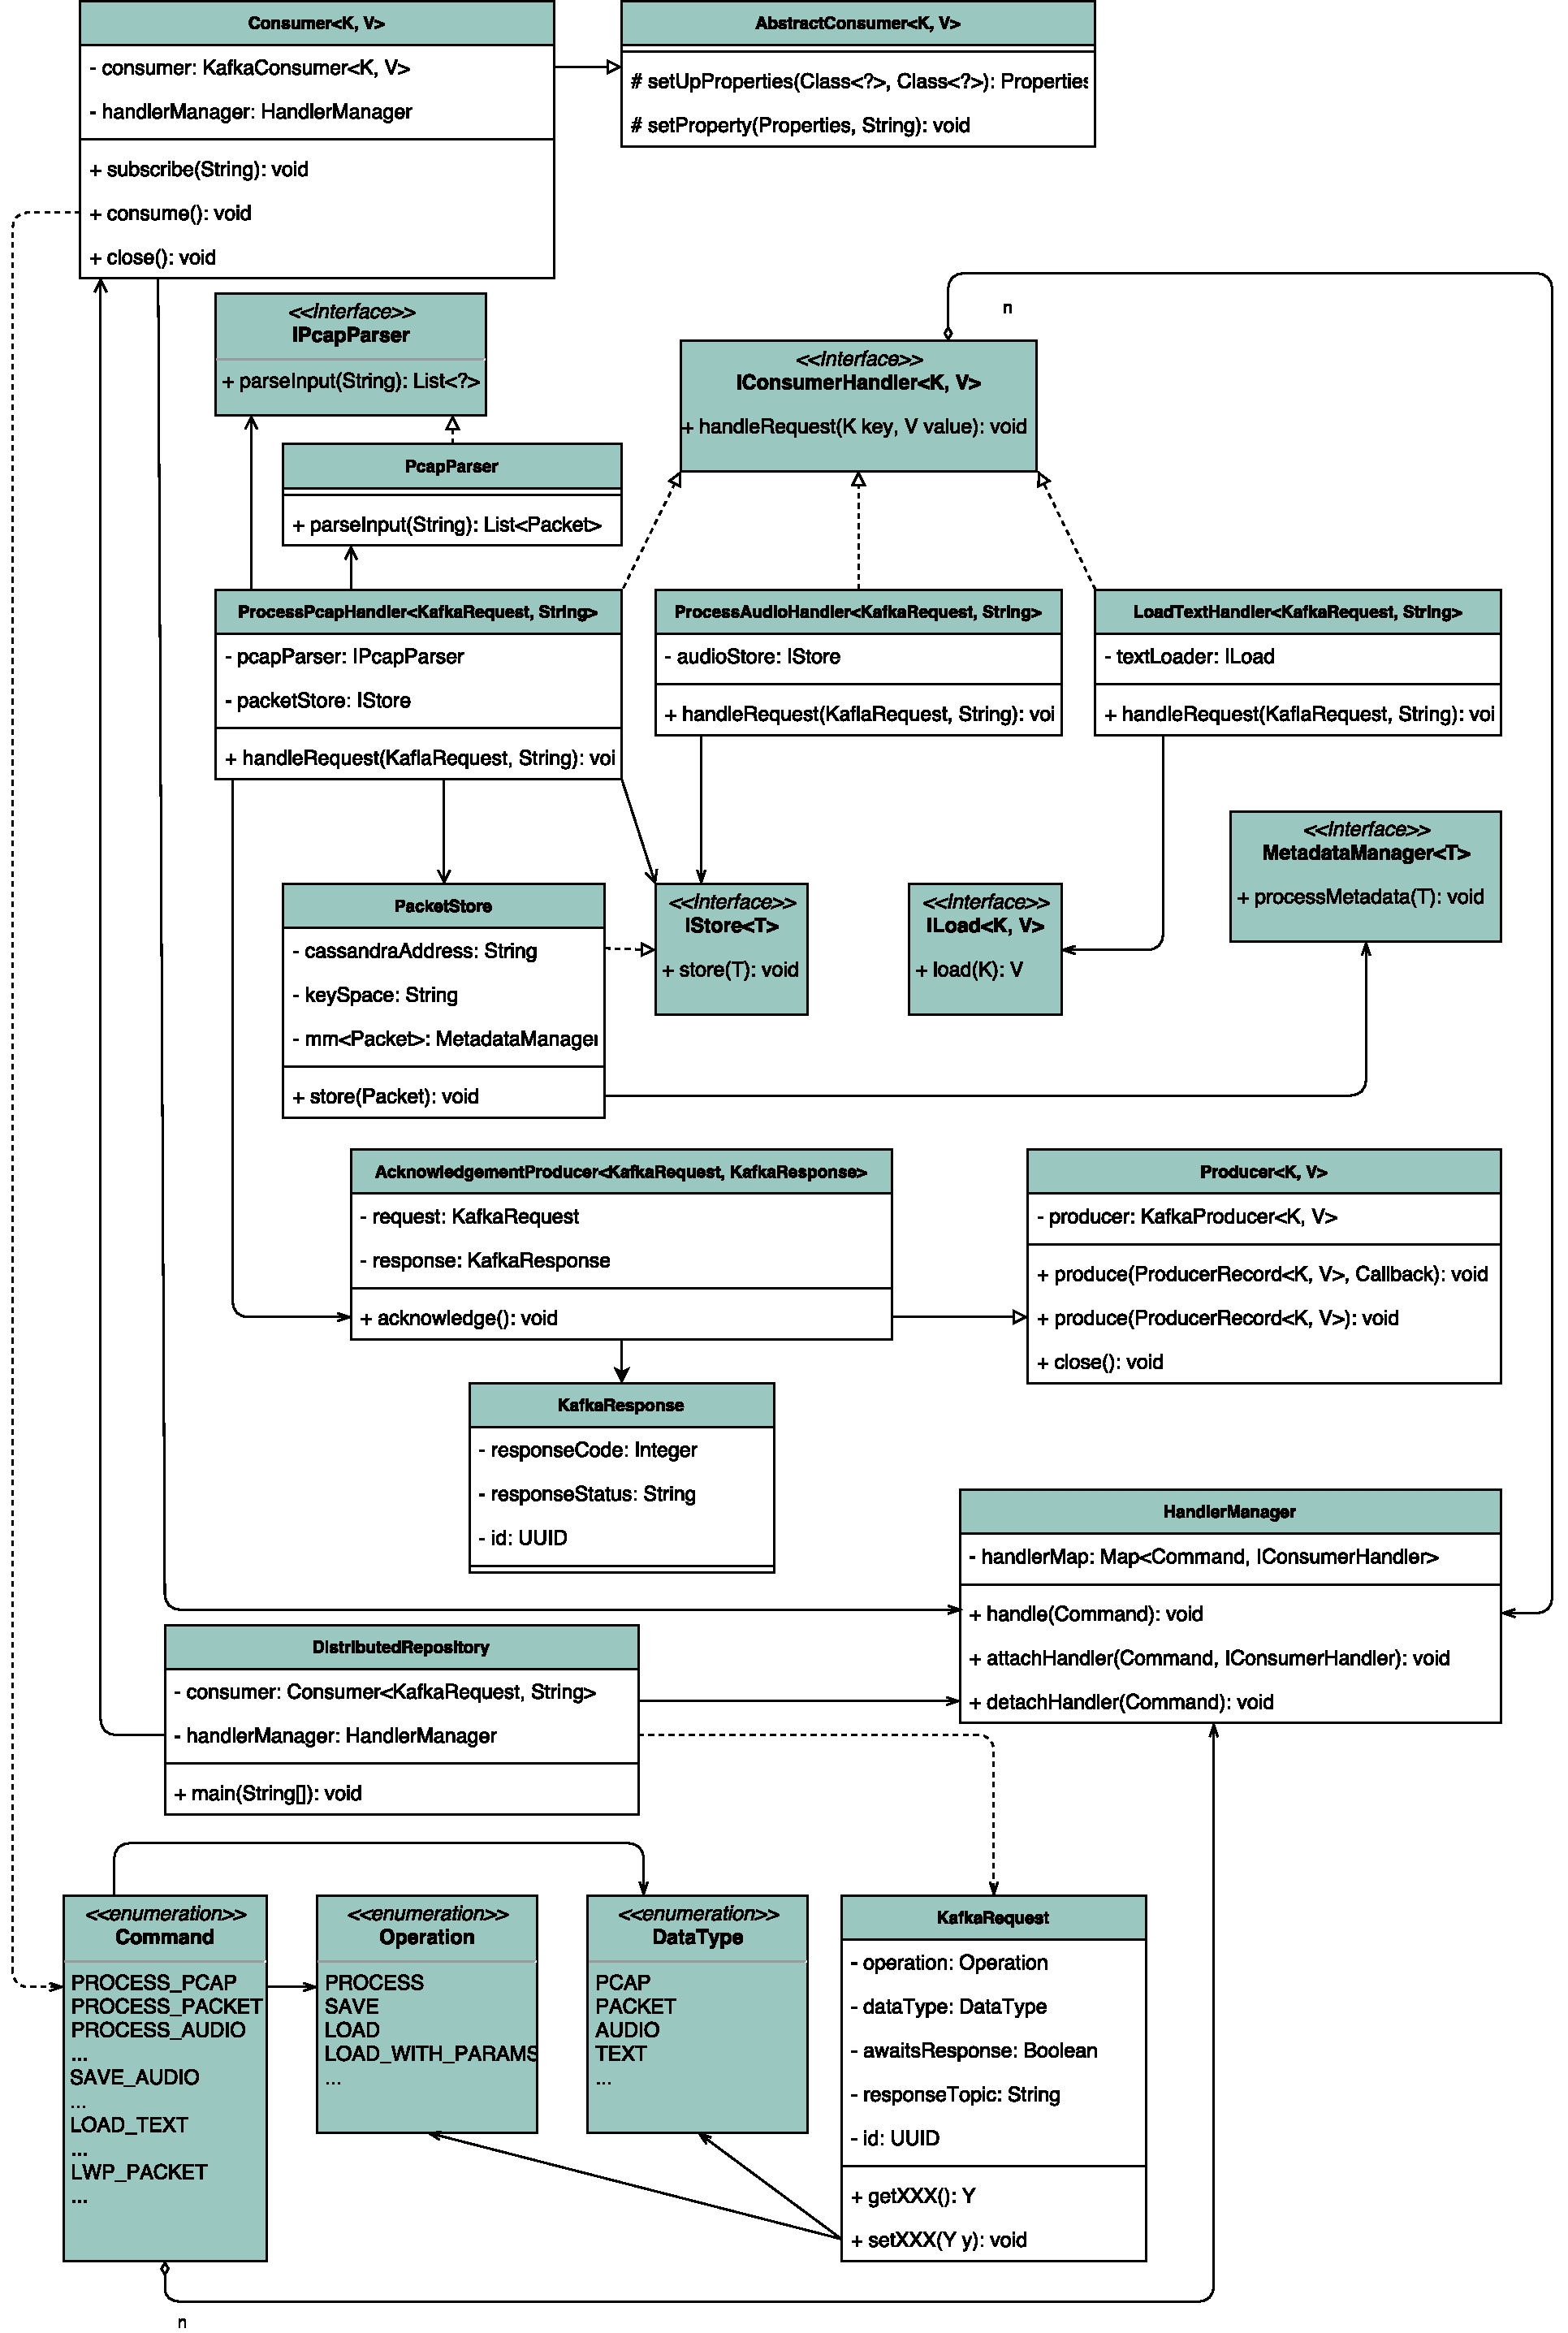
\includegraphics[width=15cm]{template-fig/Prototype_ClassDiagram.pdf}
  \caption{Diagram tříd systému.}
  \label{FIG_SystemArchitecture}
\end{figure}

\chapter{Implementace prototypu} \label{chapterPrototype}
Prototyp distribuovaného repositáře byl implementován za účelem ověření základních aspektů návrhu, k~ověření komunikace mezi klientem a~systémem, zpracování příkazů, a~také výkonu.

Prototyp má omezenou funkcionalitu co se týká zpracování různých druhů digitálních forenzních dat a~z~hlediska operací. Neobsahuje také ani systém metadat. Podporuje pouze operaci uložení a~pro soubory typu PCAP.

Klient tedy může odeslat příkaz pro operaci \texttt{SAVE} a~typ dat \texttt{PCAP}. Konzument zpráv zprávu přijme a~spustí odpovídající handler. Jak bylo výše uvedeno, soubory typu PCAP lze považovat za strukturovaná data. Handler tedy soubor rozdělí na jednotlivé pakety a~ty jsou potom serializovány a~uloženy do Cassandry. Klientovi je odeslána odpověď informující o~dokončení. Systém využívá knihovnu \texttt{pcap4j}\footnote{https://github.com/kaitoy/pcap4j} pro rozdělení na pakety.

\section{Výkon}
Tato sekce se věnuje shrnutí výkonnosti implementovaného prototypu. Test rychlosti byl proveden na této konfiguraci:

\vspace{0.5cm}
\noindent
\texttt{CPU: Intel Core i5-4200U 1.6Ghz @ 2.3Ghz} \\
\texttt{RAM: 8 GB} \\
\texttt{OS: Windows 8.1} \\
\texttt{Kafka, Zookeeper and Cassandra: running as containers in Docker environment} \\
\texttt{hosted by boot2docker}

\vspace{0.5cm}
\noindent
Pro testování byly použity PCAP soubory obsahující od stovkek paketů po několik tisíc. Tabulka \ref{TablePerformance} obsahuje informace z~měření. První sloupec udává velikost PCAP souboru v~bytech, druhý sloupec obsahuje počet paketů na daný PCAP soubor a~třetí sloupec zobrazuje průměrnou velikost paketu. Čas uvedený ve čtvrtém sloupci je měřen od odeslání příkazu od klienta po obdržení odpovědi z~repositáře. Poslední pátý sloupec udává počet paketů zpracovaných za sekundu. Pro test PCAP souborů větších než 30 MB (obsahujících přes 100 tisíc paketů) už výše uvedená konfigurace nestačila. Po několika minutách aplikace zhavarovala pro nedostatek paměti RAM.

Z~výše uvedené hardwarové konfigurace vyplývá, že nebylo využito maximálního potenciálu použitých technologií, a~to zejména distribuovanosti systému, který by běžel místo jednoho počítače v~clusteru. V~takovém prostředí by byla výkonnost systému znatelně vyšší.

\begin{figure}[!h]
  \centering
  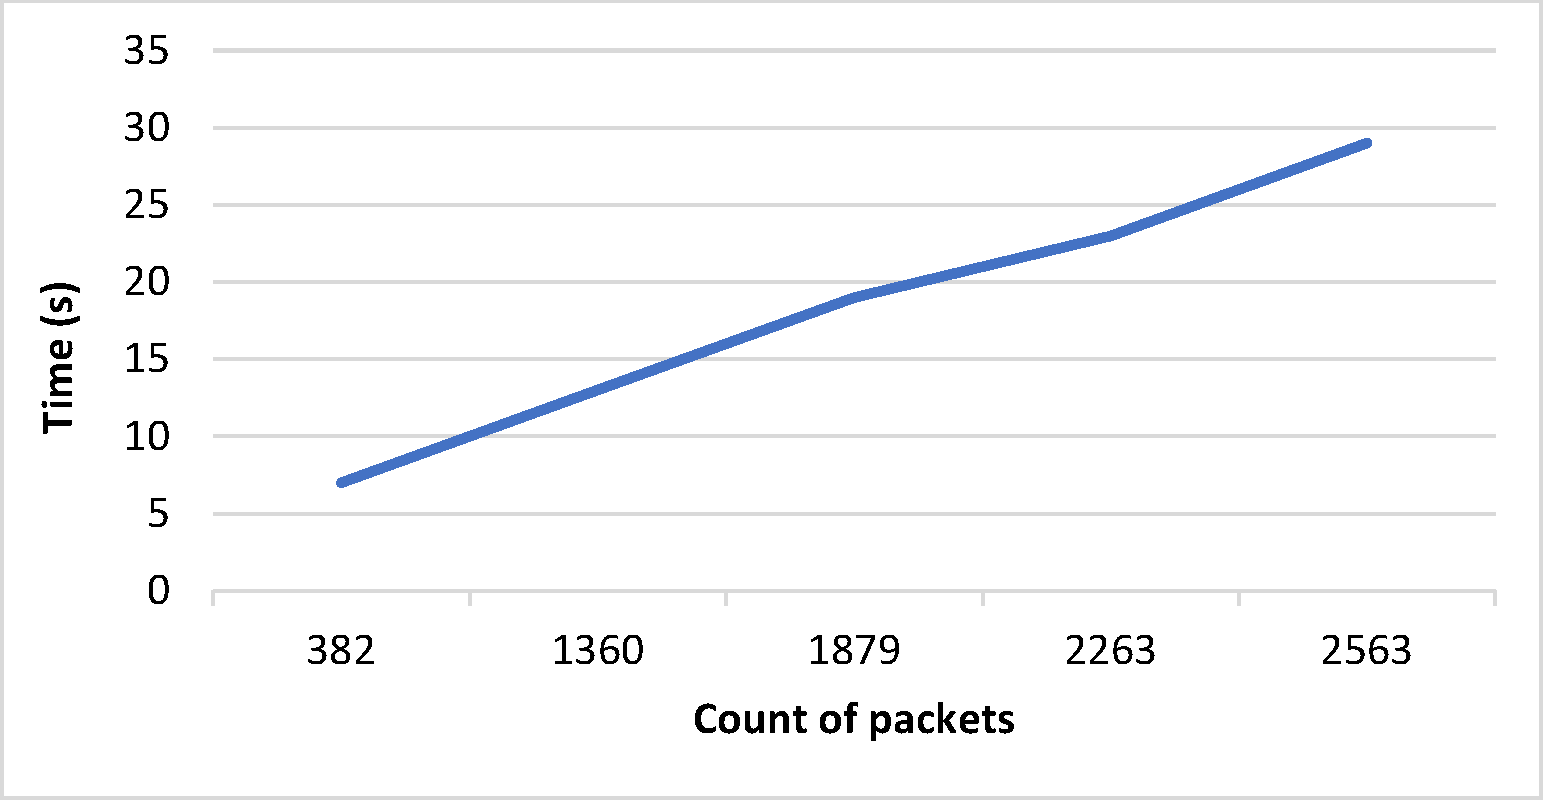
\includegraphics[width=15cm]{template-fig/PerformanceChart.pdf}
  \caption{Graf zobrazující počet uložených paketů z~jednoho PCAP souboru za čas.}
  \label{FIG_PerformanceChart}
\end{figure}

\vspace{0.5cm}

\noindent Z uvedeného grafu \ref{FIG_PerformanceChart} vyplývá lineární složitost. Podle údajů v~tabulce \ref{TablePerformance} lze průměrně zpracovat 89 paketů za sekundu při průměrné velikosti jednoho paketu 450 bytů.

%AVG time (s)	AVG packet size (Bytes)
%88,97043294	451,4784279


\vspace{0.5cm}

\begin{table}[h!]
    \centering
    \begin{tabular}{| l | l | l | l | l |}
    \hline
    PCAP size (bytes)   &   Count of packets   &   Avg. packet size &  Time (s) &   Packets/s \\ \hline
    91 340 & 382 & 239,1099476 & 7 & 54,57142857 \\ \hline
    1 955 172 & 1360 & 1437,626471 & 13 & 104,6153846 \\ \hline
    412 254 & 1879 & 219,4007451 & 19 & 98,89473684 \\ \hline
    420 869 & 2263 & 185,9783473 & 23 & 98,39130435 \\ \hline
    449 234 & 2563 & 175,276629 & 29 & 88,37931034 \\ \hline
    \end{tabular}\par
    \bigskip
    \caption{Tabulka obsahuje měřená data.}
    \label{TablePerformance}
\end{table}

\chapter{Implementace} \label{chapter_impl}

\section{Rozhraní pro dotazování dat}

\section{Moduly, knihovny a frameworky}
% TODO: \section{Architektura}
Repositář je komplexní distribuovaný systém, který je postaven na frameworku Spring, sestávající z několika modulů a knihoven. V této sekci je uvedeno, jak byl systém dekomponován do modulů a jaké knihovny byly zvoleny. Pro správu závislostí a sestavení aplikace byl zvolen nástroj \texttt{Maven}.

\vspace{0.5cm}

\noindent Pro přehled byly využity tyto knihovny a frameworky: \texttt{Spring Boot}, \texttt{Spring Data}, \texttt{Spring Kafka}, \texttt{Spring Hadoop}, \texttt{Pcap4J}, a samozřejmě ovladače pro jednotlivé databáze.

\begin{figure}[!h]
  \centering
  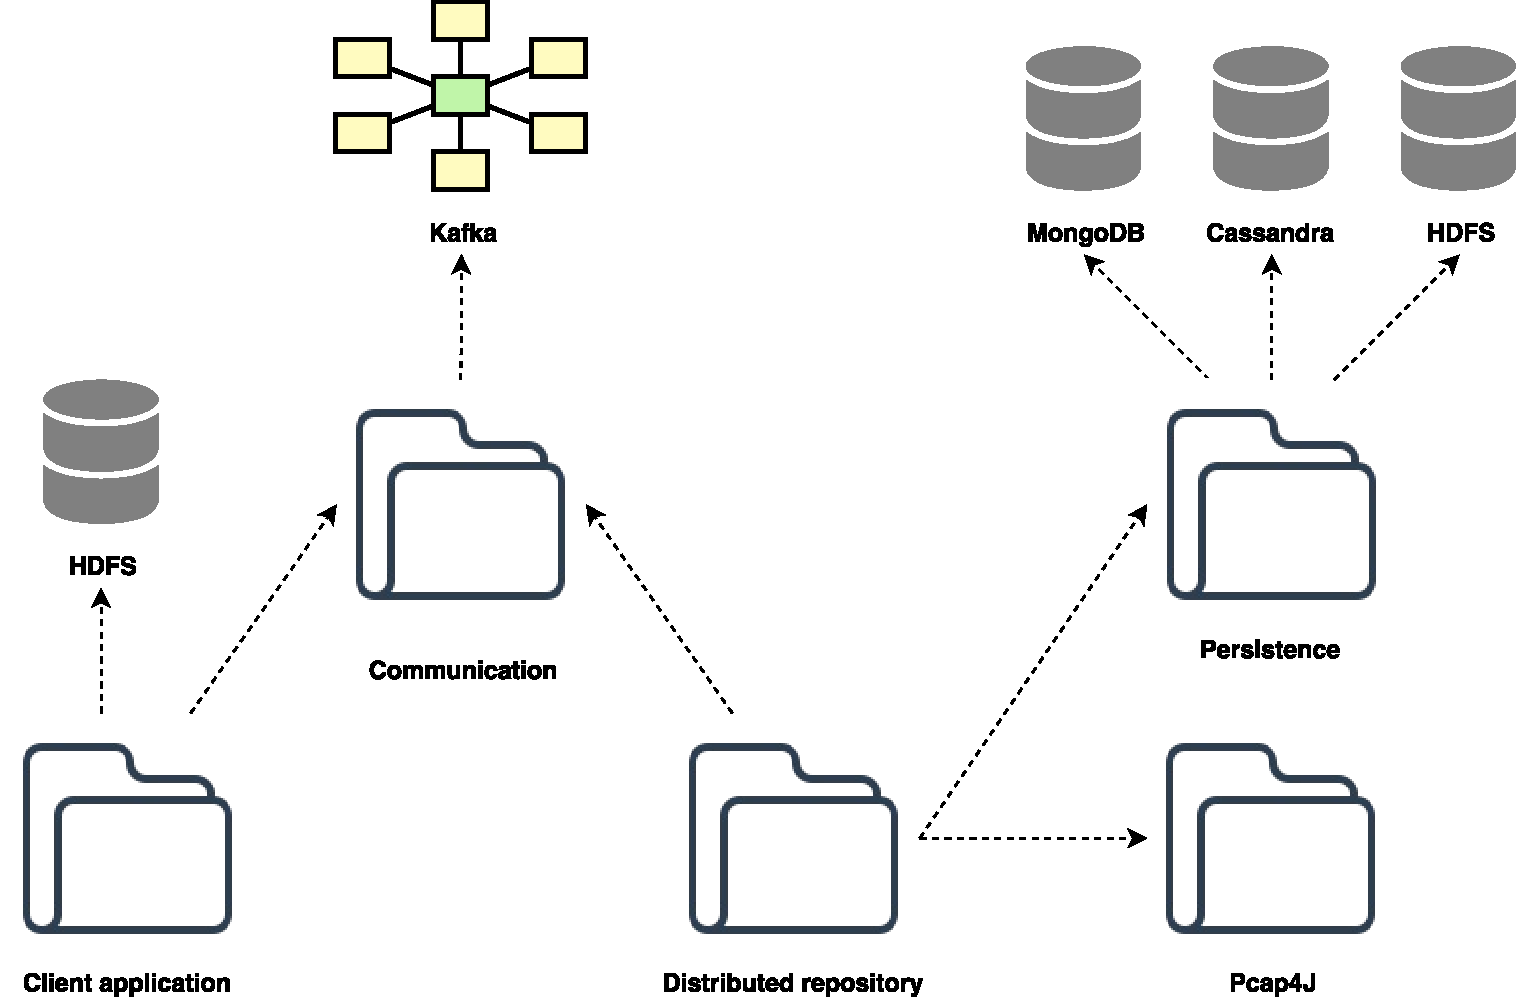
\includegraphics[width=15cm]{template-fig/Architecture.pdf}
  \caption{Schéma závislostí systému.}
  \label{FIG_Architecture}
\end{figure}

\subsection{Pcap4J}
Jedná se o knihovnu pro jazyk Java pro zachytávání, sestrojení a odesílání paketů. Knihovna je stále ve vývoji. Pcap4J pracuje nad nativní knihovnou (\texttt{libpcap}, \texttt{WinPcap}, nebo \texttt{Npcap} v závislosti na operačním systému) přes JNA (\texttt{Java Native Access})
%\footnote{https://github.com/java-native-access/jna}
a poskytuje aplikační rozhraní pro jazyk Java. Mimo výše uvedené činnosti dokáže pracovat s PCAP soubory, vytvářet a parsovat je na jednotlivé pakety. Každý paket implementuje rozhraní \texttt{Packet}. Toto rozhraní nabízí mimo jiné dvě klíčové metody \texttt{contains} a \texttt{get}. Metoda \texttt{contains} slouží ke kontrole, jestli je paket konkrétního typu, který chceme získat. Metoda má jako parametr třídu, které je paket typem, hlavička metody potom vypadá:

\vspace{0.5cm}
\texttt{boolean contains(Class<T> clazz)}

\vspace{0.5cm}
\noindent Ke konkrétnímu typu paketu, např. IP paketu, se přistupuje pomocí reflexe voláním metody:

\vspace{0.5cm}
\texttt{T get(Class<T> clazz)}

\vspace{0.5cm}
\noindent Tedy například:

\vspace{0.5cm}
\texttt{IPv4Packet ipv4Packet = ethernetPacket.get(IPv4Packet.class);}

\vspace{0.5cm}
\noindent Návratová hodnota metody \texttt{get} je objekt třídy uvedené v parametru. Před voláním \texttt{get} je vhodné zkontrolovat typ pomocí metody \texttt{contains}. Z konkrétního paketu už lze získávat potřebné informace, v případě IP paketu údaje z hlavičky jako zdrojová a cílová IP adresa, verze protokolu apod. Analogicky lze postupovat i v případě ostatním typů paketů, Z TCP paketu lze získat údaje o portech, sekvenční čísla, checksum a další.

Knihovna reflektuje zapouzdření, které spočívá ve vložení protokolové datové jednotky (anglicky \texttt{Protocol Data Unit}) vyšší vrstvy do protokolové jednotky nižší vrstvy. Takže ethernetový paket může být současně i IP paketem a podobně.

\begin{figure}[!h]
  \centering
  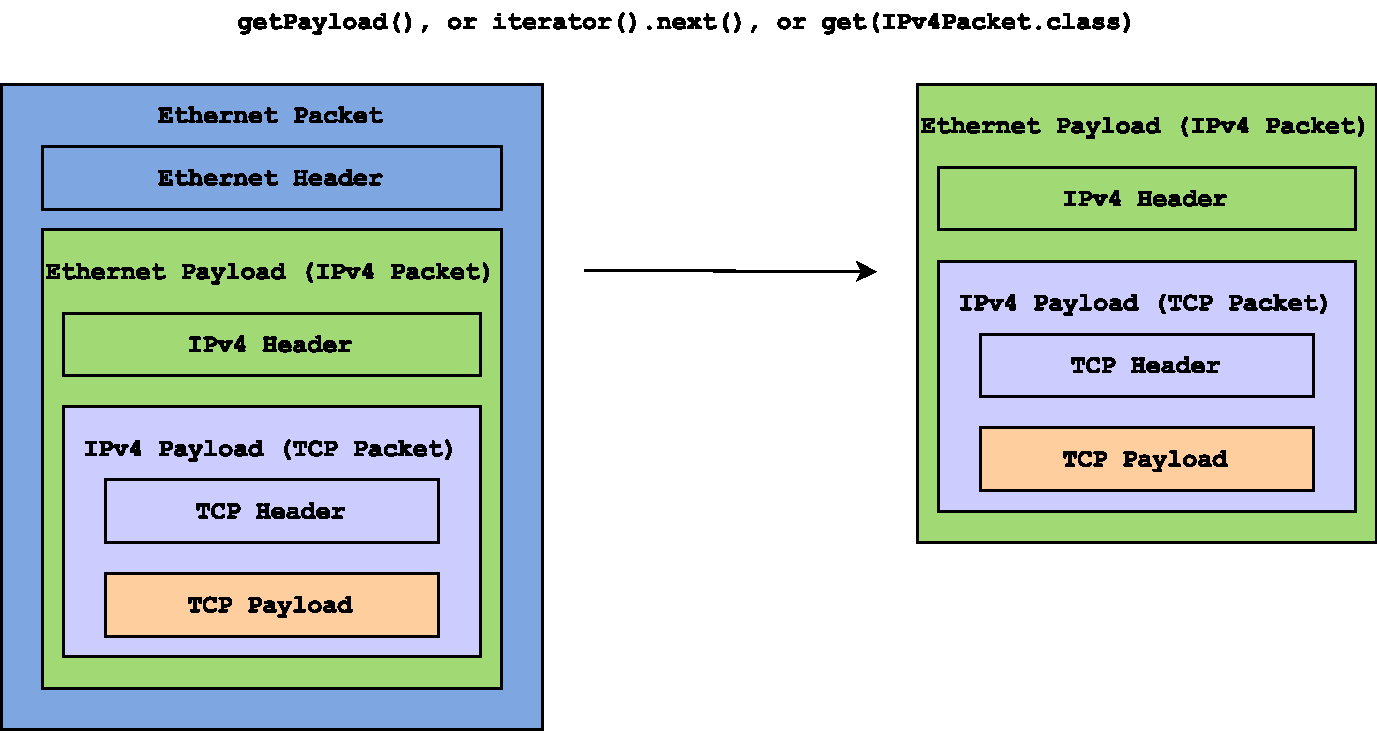
\includegraphics[width=14.8cm]{template-fig/Pcap4JExample.pdf}
  \caption{Schéma znázorňující výše uvedený příklad pro manipulaci s pakety \cite{gitPcap4J}.}
  \label{FIG_Architecture}
\end{figure}

\section{Úložiště}
Jak už bylo uvedeno v kapitole \ref{distrRepDesignChapter}, úložiště je tvořeno NoSQL databázemi Cassandra a MongoDB, a distribuovaným souborovým systémem HDFS. Zatímco předešlá kapitola jen nastínila vlastnosti těchto úložišť, zde budou vysvětleny technické detaily a práce s nimi.

\subsection{Cassandra}

\subsubsection{Asynchronní dotazy}
Distribuovaný repositář komunikuje s databází asynchronně z důvodu co největší propustnosti a rychlosti. Asynchronní komunikace je umožněna díky třídám a metodám ovladače pro jazyk Java od společnosti DataStax, který je stále ve vývoji \footnote{https://github.com/datastax/java-driver}. Tento ovladač používá asynchronní architekturu. Takový způsob komunikace dovoluje klientské aplikaci ukládat data a provádět nad nimi dotazy neblokujícím způsobem, díky tzv. \texttt{Future} instancím \cite{asyncQueriesCassandra}.

\begin{figure}[!h]
  \centering
  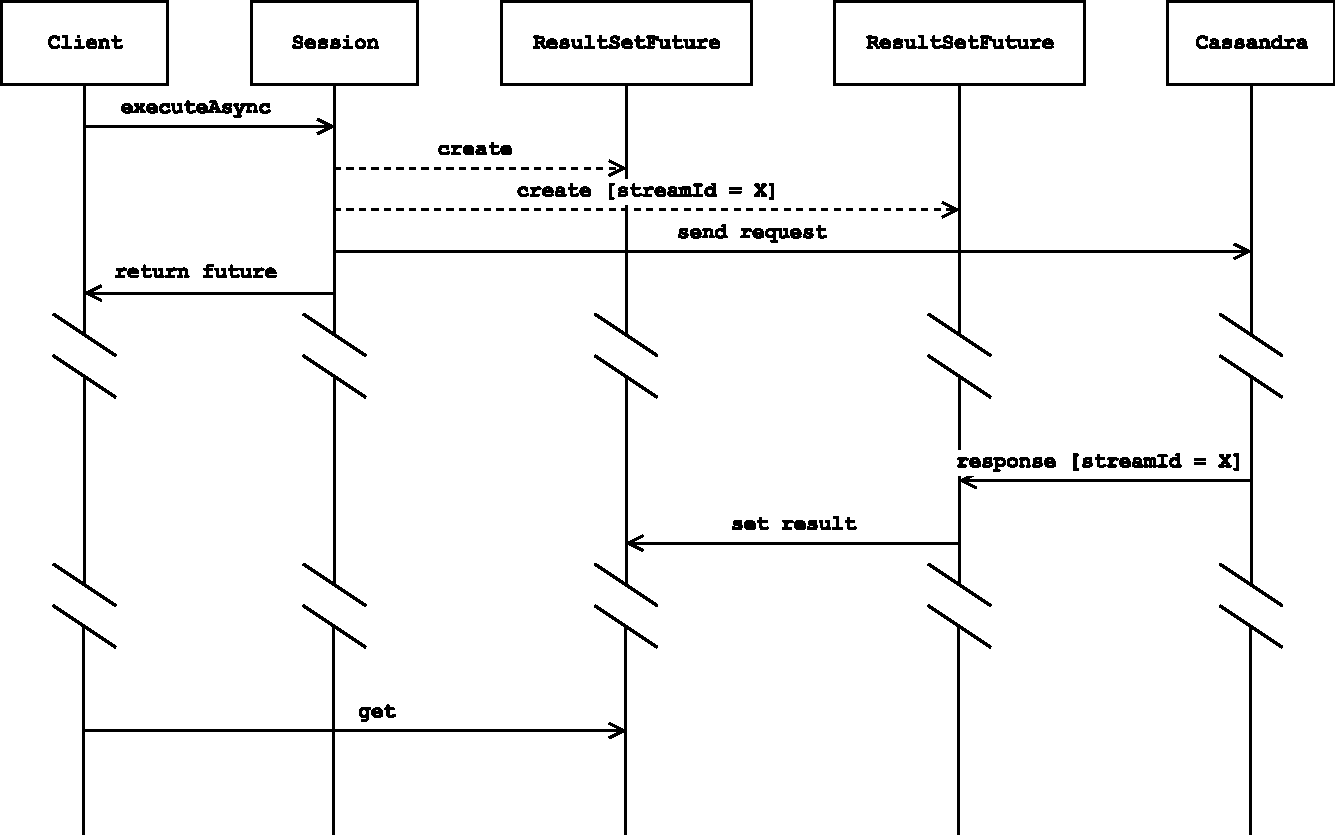
\includegraphics[width=15cm]{template-fig/CassandraAsyncQueries.pdf}
  \caption{Sekvenční diagram znázorňující jednotlivá volání metod při vykonávání asynchronního dotazu do databáze Cassandra \cite{asyncQueriesCassandra}.}
  \label{FIG_Architecture}
\end{figure}

\noindent Kromě zaslání dotazu do databáze, ovladač registruje interní obsluhu v podobě objektu \texttt{ResponseHandler}, který zpracuje odpověď dotazu, až bude k dispozici. Po zaregistrování obsluhy je předáno řízení vykonávání volajícímu programu společně s objektem třídy \texttt{ResultSetFuture}, pomocí kterého klient dokáže získat výsledek dotazu a dále s ním pracovat.
Až databáze dotaz dokončí a vrátí odpověď, ovladač avizuje ResponseHandler (obecně může být zaregistrováno mnoho takových obsluh pro různé dotazy, párování je provedeno pomocí unikátního ID \texttt{streamId}, které bylo zasláno s dotazem). Obsluha třídy ResponseHandler dokončí volání upozorněním objektu třídy ResultSetFuture.
Klientský kód získá výsledek dotazu provedením metody \texttt{get} nad objektem ResultSetFuture. Volání této metody je blokující, pokud ještě nebyl nastaven výsledek objektu ResultSetFuture \cite{asyncQueriesCassandra}.

Čekat na výsledek blokujícím způsobem není efektivní, proto existuje i způsob bez blokování. V takovém případě musí klient k objektu ResultSetFuture zaregistrovat svůj tzv. \texttt{callback}, který bude vykonán, až bude výsledek k dispozici.
Lze zvolit i jiné vlákno pro jeho vykonání, aby aktuálně běžící kód nemusel být pozastaven. To lze například pomocí knihovny \texttt{Guava} od Google a jejich tříd \texttt{Futures} a \texttt{FutureCallback}.

Pozn: Ovladač od DataStax je obecně celý asynchronní, uvnitř jeho synchronních metod je zavolána asynchronní verze, a pak okamžitě blokující metoda get.

\subsection{MongoDB}

\subsubsection{Reaktivní dotazy}
Pro komunikaci s databází MongoDB existuje několik ovladačů, tzn. synchronní, asynchronní, a také ovladač založen na reaktivním paradigmatu. Poslední zmíněný byl využit pro distribuovaný repositář. Tento ovladač poskytuje asynchronní zpracování dotazů neblokujícím způsobem. Zcela implementuje aplikační rozhraní tzv. \texttt{Reactive Streams} \footnote{http://www.reactive-streams.org/}. Mezi silné stránky tohoto paradigmatu patří: funkcionální přístup, asynchronní zpracování chyb, jednoduchá multivláknovost \cite{oficReactiveX}. Často je prezentováno jako rozšíření návrhových vzorů Pozorovatel (angl. \texttt{Observer}) a iterátor (angl. \texttt{Iterator}). Reaktivní paradigma se samozřejmě netýká jen databází, platí obecně a lze s ním vyvíjet celé aplikace.

% https://dzone.com/articles/what-are-reactive-streams-in-java
% http://vsadnajavu.cz/2017-06/odborne/spring-framework/spring-5-0-reactive/

Manipulaci s metadaty zajišťuje tzv. reaktivní JPA (\texttt{Java Persistence API}) patřící pod projekt Spring. Tato vrstva využívá výše zmíněného reaktivního ovladače pro MongoDB. Následuje detailnější pohled na tento programovací model a aplikační rozhraní \cite{springDataReactive}.

Základem je vytvoření entitní třídy, která reprezentuje objekty ukládané do tabulky databáze nebo v tomto případě do kolekce. Pro entitní třídu lze definovat rozhraní, které představuje použití návrhového vzoru \texttt{Repository}. Výhodou je, že objekty nemají ponětí o tom, jakým způsobem jsou ukládány. O persistenci se postará Repository. Definované rozhraní představující Repository musí dědit rozhraní

\vspace{0.5cm}
\texttt{ReactiveCrudRepository<T, ID>}

\vspace{0.5cm}
\noindent se dvěma typovými parametry, kde typ \texttt{T} udává typ entitní třídy a typ \texttt{ID} udává typ unikátního ID pro záznamy dané entitní třídy. Toto rozhraní definuje doménově specifické \texttt{CRUD} metody s parametry reaktivních typů \texttt{Flux} a \texttt{Mono}, které budou vysvětleny dále. Příkladem pro manipulaci s metadaty je rozhraní:

\vspace{0.5cm}
\texttt{PacketMetadataRepository extends} \\
\indent \indent \indent \texttt{ReactiveCrudRepository<PacketMetadata, String>}

\vspace{0.5cm}
\noindent Framework Spring se postará o implementaci tohoto rozhraní pro všechny CRUD operace nabízené tímto rozhraním.

Reaktivní přístup byl zvolen hlavně z důvodu vrstvy JPA, kterou zajišťuje sám Spring. Přístup pomocí asynchronních dotazů by šel využít taktéž, ale manipulace s metadaty, ukládání a dotazování, by byla těžkopádná, potřebovala výrazně více režijního kódu, a byla by nepřehledná, protože asynchronní ovladač pracuje primárně na úrovně dokumentů vkládaných do kolekcí. S tím by souviselo manuální sestavování a parsování objektů reprezentujících dokument.

\subsubsection{Reaktivní typy}
Výchozími reaktivními typy jsou Flux a Mono pocházející z projektu \texttt{Project Reactor} (implementací reaktivních typů existuje více, další je např. \texttt{ReactiveX}). Flux slouží pro vztahy typu N, Mono pak pro vztahy typu 0 nebo 1 \cite{projectReactor}.
Reaktivní typy nejsou určeny k tomu, aby zpracovaly požadavky nebo data rychleji, ve skutečnosti představují malou režii ve srovnání s běžným blokujícím zpracováním. Jejich síla spočívá v obsluze více požadavků paralelně, a ve zpracování operací s latencemi, např. dotaz pro data z databáze nebo ze vzdáleného serveru, mnohem efektivněji. Poskytují lepší plánování zdrojů, zacházení s časem a latencemi. Na rozdíl od tradičního zpracování blokujícím způsobem, které pozastaví aktuální vlákno čekáním na výsledek operace, reaktivní aplikační rozhraní čekající na výsledek nestojí žádný čas, dotazuje se pouze na objem dat, který je schopné zpracovat. Zabývá se celými streamy dat, nikoliv pouze individuálními elementy jeden za druhým \cite{springReactiveTypes}.

Reaktivní aplikační rozhraní poskytuje operátory podobné streamům z jazyka Java, ale tyto operátory pracují obecně s jakoukoliv sekvencí, nejsou omezeny pouze na kolekce, a umožňují definovat řetězec transformačních operací, které se aplikují na data procházející streamem. Streamy dokáží zpracovat synchronní i asynchronní operace, data lze řetězit, sloučit, nebo na ně aplikovat různé transformace \cite{springReactiveTypes}.

Implementace reaktivního rozhraní je založena na výše zmíněné specifikaci Reactive Streams. Základním kamenem jsou čtyři rozhraní \texttt{Publisher}, \texttt{Subscriber}, \texttt{Subscription} a \texttt{Processor}. Jejich zodpovědnosti jsou:
\begin{itemize}
    \item Publisher - poskytovatel potenciálně neomezeného počtu elementů v sekvenci, odesílá je podle požadavků obdržených od svých příjemců. Může obsluhovat dynamicky v čase mnoho příjemců.
    
    \item Subscriber - příjem elementů od poskytovatele, na elementy se dotáže sám. Typicky má tyto 3 metody: \texttt{onNext} - zpracování elementu, \texttt{onError} - zpracování chyby, a \texttt{onComplete} - signalizace dokončení operace onNext.
    
    \item Subscription - může být použito pouze jedním příjemcem. Představuje jednotku přijetí elementu od poskytovatele k odběrateli.
    
    \item Processor - procesory jsou speciálním případem poskytovatele, který je zároveň příjemcem \cite{reactoreRefGuide}. Reprezentují jednotku vykonávání.
\end{itemize}

\noindent Reaktivní typy Flux a Mono implementují rozhraní poskytovatele. Současně umožňují přidávat transformační operace ke každému elementu sekvence. Jednoduché je i zpracování chyb asynchronním způsobem bez použití bloků \texttt{try} a \texttt{catch}. Klientský kód se chová jako odběratel.

\subsection{HDFS}

\section{Logování}

\section{Zpracování chyb}

\chapter{Výkon} \label{chapter_performance}

\chapter{Závěr}
V~rámci semestrálního projektu jsem se seznámil s~formáty digitálních forenzních dat a~způsoby jejich uložení. Prozkoumal jsem existující systémy pro uložení digitálních forenzních dat (včetně AFF4). Seznámil jsem se s~distribuovanými databázemi a~NoSQL databázemi. Navrhl jsem distribuované úložiště rozsáhlých digitálních forenzních dat včetně aplikačního rozhraní.

Pro ověření základních aspektů návrhu jsem také implementoval prototyp distribuovaného repositáře, který realizuje rozhraní komunikace s~klientem, způsob ovládání repositáře, a~rovněž zpracovává požadavky od klienta. Provedl jsem také základní vyhodnocení z hlediska výkonnosti na běžně dostupné hardwarové konfiguraci.

Dalším krokem bude rozšíření implementace prototypu o~podporu nových druhů digitálních forenzních dat, zejména zjednodušení přidávání nových akcí, které zpracovávají příkazy od klienta. Bude také implementován podsystém metadat, který bude provádět předzpracování dat.
Implementovaný systém bude zhodnocen z~hlediska výkonu a~použití pro vybrané druhy digitálních forenzních dat.

%=========================================================================
